\documentclass[a4paper,twoside,10pt]{report}

\usepackage{mathtools}
\usepackage{amssymb,amsmath}

% Pranav comment this line below to take out all the comments from the paper
\newcommand{\ENABLECOMMENTS}{}
\usepackage[T1]{fontenc}
\usepackage{ifpdf}
\usepackage{url}
\usepackage{tabularx}
\ifpdf
\usepackage[pdftex]{graphicx}
\graphicspath{{figs/}}
\DeclareGraphicsExtensions{.pdf,.png,.jpg}
\else
\usepackage[dvips]{graphicx}

\graphicspath{{eps/}}
\DeclareGraphicsExtensions{.eps}
\fi
\usepackage{float}
%\usepackage[caption=false,font=footnotesize]{subfig}
\usepackage[font=footnotesize]{caption}
\usepackage{subcaption}
\captionsetup{compatibility=false}
\usepackage{setspace}
\usepackage{balance}
\pdfminorversion=6
\hyphenation{op-tical net-works semi-conduc-tor}
\newcommand{\indentitem}{\setlength\itemindent{0pt}}
\usepackage{algorithmic}
\usepackage{algorithm}
\newcommand{\algorithmicinput}{\textbf{Input:}}
\newcommand{\INPUT}{\item[\algorithmicinput]}
\newcommand{\algorithmicoutput}{\textbf{Output:}}
\newcommand{\OUTPUT}{\item[\algorithmicoutput]}
\renewcommand{\algorithmicrequire}{\textbf{Pre Condition:}}
\renewcommand{\algorithmicensure}{\textbf{Post Condition:}}
\floatname{algorithm}{Procedure}
\usepackage{tikz}
\usetikzlibrary{matrix,arrows,circuits.ee,circuits.ee.IEC,shapes.geometric,shapes.misc}
\newcommand{\iap}{\textit{DREMS}}
%\newcommand{\iapfull}{\textbf{D}istributed \textbf{S}oftware \textbf{P}latform }
\newcommand{\iapfull}{\textbf{D}istributed \textbf{RE}altime \textbf{M}anaged \textbf{S}ystem}% Algorithmic modifications
\newcommand{\ALOOP}[1]{\ALC@it\algorithmicloop\ #1%
  \begin{ALC@loop}}
\newcommand{\ENDALOOP}{\end{ALC@loop}\ALC@it\algorithmicendloop}
\renewcommand{\algorithmicrequire}{\textbf{Input:}}
\renewcommand{\algorithmicensure}{\textbf{Output:}}
\newcommand{\algorithmicbreak}{\textbf{break}}
\newcommand{\BREAK}{\STATE \algorithmicbreak}
\usepackage{color}

\ifdefined\ENABLECOMMENTS
\newcommand{\AD}[1]{{\texttt{\color{red}AD:#1}}}
\else
\newcommand{\AD}[1]{}
\fi
\newenvironment{noindlist}
 {\begin{list}{\labelitemi}{\leftmargin=0.1em \itemindent=0em \itemsep=0.3em}}
 {\end{list}}
\usepackage{multirow}
\begin{document}
\title{F6 Timing Analysis \\ Users Guide}
\author{Pranav Srinivas Kumar \\ Email: pkumar@isis.vanderbilt.edu}
\maketitle
\tableofcontents
\chapter{Introduction}
\label{chapter:introduction}

The decisive role of optimized and robust software in safety and mission-critical distributed real-time embedded (DRE) systems is becoming increasingly recognized. Embedded software is pertinent in a variety of heterogeneous domains e.g. avionics \cite{burke2010distributed}, automotive systems \cite{navet2008automotive}, locomotives \cite{zimmermann2003train}, and industrial control systems \cite{zoitl2008real}. The volume and complexity of such software grows everyday depending on an assortment of factors, including challenging system requirements e.g. resilience to hardware and software faults, remote deployment and repair. Deployment, the procedure for launching or reconfiguring software processes on embedded hardware, becomes extremely difficult if obtaining access to such devices is limited. Large scale deployment of embedded software, for this reason, has become considerably more arduous -- periodic peer reviews, numerous verification and certification methods are applied to maintain industry standards for safety, precision and reliability of embedded real-time software. Even still, software errors manifest in deployed systems; errors that can be extremely difficult to reproduce in a laboratory test environment. 

There exists a long list of real-world scenarios where errors in embedded software implementations has cost millions of dollars and human life. Between 1999 and 2010, at least 2,200 Toyota vehicles sold in the United States experienced unintended cases of rapid acceleration, causing nearly 900 accidents and over 100 deaths \cite{Cusumano:2011:RTD:1866739.1866750}. In 2010, Toyota recalled some 10 million vehicles, an extraordinary number given that the company sold only about seven million vehicles during that period. Toyota engineers described the problem as a disconnect in the vehicle's complex anti-lock brake system (ABS) that causes less than a one-second lag in its operation. With this delay, a vehicle going 60 mph will have traveled nearly another 90 feet before the brakes begin to take hold. Brakes in Toyota hybrids such as the Prius operate differently from brakes in most cars. In addition to the standard brakes, which use friction from pads pressed against rotors, the embedded software driving the electric motors help slow the vehicle. This process also generates electricity to recharge the batteries. This is a prime example of how timing errors in consumer-focused embedded software, spanning millions of lines of code, can have disastrous effects to everyday life. The Prius is Toyota's third best-selling model in the United States. The automaker recalled 2.3 million vehicles on January, 2011 because of problems with sticking gas pedals and later halted the sale of the eight models involved in the recall. Toyota's U.S. sales plunged 16 percent in January as a result, even as sales of other automakers rose.

To mitigate such software complexity, model-driven component-based software engineering (CBSE) and development \cite{beydeda2005model, heineman2001component, clemens1998component, simulink1993mathworks, autosar} has become an accepted practice. CBSE tackles escalated demands with respect to requirements engineering, high-level design, error detection, tool integration, verification and maintenance. The widespread use of component technologies in the market has made CBSE a focused field of research in the academic sectors. Applications are built by assembling together small, tested component building blocks that implement a set of services. These building blocks are typically built from UML \cite{UML} class diagrams, or imported from other projects/vendors and \emph{connected} together via exposed interfaces, providing a "black box" approach to software construction. This approach also treats software verification in a more modular fashion; the various software components can be verified individually and then composed together to derive a functional system. 

Remote embedded devices e.g. fractionated spacecraft \footnote{A fractionated spacecraft is a satellite architecture where the functional capabilities of a conventional monolithic spacecraft are distributed across multiple modules which interact through wireless network links.} following mission timetables and hosting distributed software applications expose several concerns including strict timing requirements, complexity in deployment, repair and integration; and resilience to faults, including mechanical failures like surface fractures, electrical failures such as single-event upsets, and manufacturing defects, and lastly software failures such as design defects and run-time faults. High-security and time-critical software applications hosted on such platforms run concurrently with all of the system-level mission management and fault recovery tasks that are periodically undertaken on the distributed nodes. Once deployed, it is often difficult to obtain a reliable period of low-level access to such remote systems for runtime debugging and evaluation. These types of DRE systems, therefore demand comprehensive design-time modeling and analysis methods to detect possible anomalies in system behavior, like the unacceptable response times in the advanced braking systems in vehicles. 

With the DARPA System F6 Project, our team has designed and prototyped a full information architecture called \emph{\textbf{D}istributed \textbf{RE}al-time \textbf{M}anaged \textbf{S}ystems} (DREMS) \cite{ISIS_F6_Aerospace:12,DREMS13Software} that addresses requirements for rapid component-based application development and deployment for fractionated spacecraft. The stack of developed software includes a  design-time model-driven development tool suite \cite{ISIS_F6_SFFMT:13}, and a component model \cite{ISIS_F6_ISORC:13} with precise execution semantics enabling robust and analyzable software designs. The minutiae of the DREMS architecture are described in Chapter \ref{chapter:DREMS}. The formal modeling and analysis methodology presented in this dissertation focuses on applications that rely on this foundational architecture. 

The principle behind design-time analysis here is to map the structural and behavioral specifications of the system under analysis into a formal domain for which analysis tools exist. The key is to use an appropriate model-based abstraction such that the mapping from one domain to another remains valid under successive refinements in system development such as code generation. The analysis must ensure that as long as the assumptions made about the system hold, the behavior of the system lies within the safe regions of operation. The results of this analysis will enable system refinement and re-design if required, before actual code development. 

\begin{figure}
	\centering
	\begin{subfigure}{.5\textwidth}
		\centering
		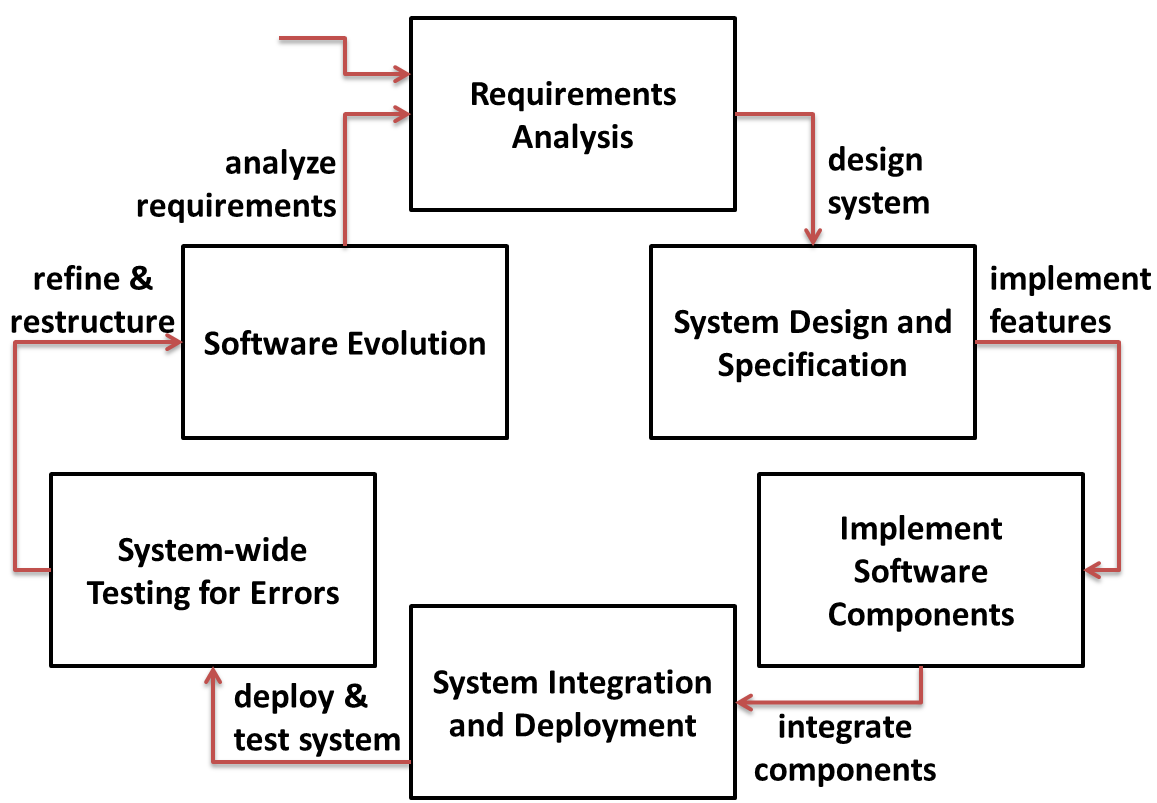
\includegraphics[width=0.9\linewidth]{sdlc}
		\caption{Industrial SDLC}
		\label{fig:sdlc}
	\end{subfigure}%
	\begin{subfigure}{.5\textwidth}
		\centering
		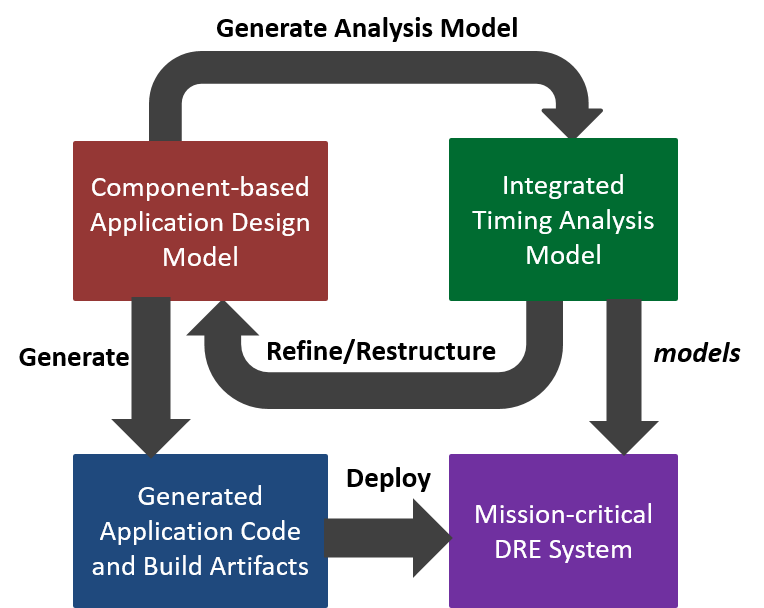
\includegraphics[width=\linewidth]{big_picture_2}
		\caption{DREMS Analysis-driven Workflow}
		\label{fig:big_picture}
	\end{subfigure}
	\caption{Embedded Software Development Lifecycle Comparison}
	\label{fig:test}
\end{figure}

Figure \ref{fig:sdlc} shows a \emph{spiral model} \cite{boehm1988spiral} of a typical industrial software/system development life cycle (SDLC). The five stages in this cycle include requirements analysis, software design, implementation, integration testing, and design evolution. Although the intricacies of each stage is hidden, the large majority of industrial software development follows this lifecycle. Embedded software development, especially for safety critical systems, does not lend itself well to this life cycle, mainly because the deliverable in such projects is usually not just a software package or a hardware platform but an amalgamation of both. Software development in fields like robotics, is tightly coupled with the hardware; assessment of software performance is sometimes dependent on and blocked by the hardware availability. Such blocking delays lead to inefficiencies in software evaluation and longer development times. It is also possible that design oversights could lead to poor timing performance e.g. long response times to critical events, that could damage the hardware in the process. Thus, the analysis presented in this work, supports and argues for a verification-driven workflow, as shown in Figure \ref{fig:big_picture}. The software evaluation is performed at design-time and as often as possible until the assembly is refined and optimized. Application developers use domain-specific modeling languages to structure large-scale component assemblies and modular code generation features to speed up software development efforts. Moreover, domain-specific properties such as interaction patterns, component execution code, and associated temporal properties such as worst-case execution times, deadlines etc. can be easily injected into such models. Using such application parameters in the \textit{design} model, a Colored Petri net-based (CPN) \cite{CPN} \textit{formal analysis model} is generated. The system behavior is both simulated and analyzed using a CPN execution engine, CPN Tools \cite{CPNTools}, and useful properties of the system are verified. By generating a bounded \emph{state space} of the system, the execution traces exhibited by the system are searched for property violations. Such system properties include the lack of deadlocks, deadline violations and worst-case trigger-to-response times. The goal of this analysis is to ensure that a component-based system: an assembly of tested component building blocks, meets the temporal specifications and requirements of the system.  

The results of this analysis will help improve the structure of the application, enabling safe deployment of dependable components that are known to operate within system specifications. Using CBSE also enables this restructuring process as the components are not tightly coupled software entities. So, when designing the integrated system, the analysis can be performed by assigning \emph{time budgets} to the discrete tasks in the execution. This enables timing analysis before implementation and also uses the time budgets as requirements for efficient code implementation. These budgets are often derived from some high-level requirements and appropriately distributed between the different components in the system. The analyzed system may not necessarily be complete, but instead be in a process of evolution. As the design progresses, the system requirements become concrete and the design is re-verified at each stage to ensure the consistency of all timing guarantees. 

The remainder of this dissertation is organized as follows. Chapter \ref{chapter:fundamentals} describes some fundamental concepts about distributed real-time systems, component-based software and some challenges in timing analysis. Chapter \ref{chapter:related-research} briefly describes general software testing and analysis methodologies, and summarizing related research in timing analysis and verification for distributed real-time embedded applications. Chapter \ref{chapter:DREMS} introduces the DREMS infrastructure and the Component Model used to experiment with and validate the timing analysis results. Chapter \ref{chapter:modeling} discusses the Colored Petri net-based timing analysis model devised for component-based DRE systems. Chapter \ref{chapter:analysis} describes the scope and efficiency of the analysis methods implemented with this CPN model. Chapter \ref{chapter:evaluation} evaluates this model with published results on analysis design, scalability and experimental validation. Finally, Chapter \ref{chapter:conclusion} concludes the dissertation, providing a summary of the detailed work and describing potential future work.
\chapter{Modeling Component Operations}

In order to describe the modeling and analysis aspects of this tool, consider the following example: 

\section{Trajectory Planning Application}

The component assembly for this application is shown in Figure \ref{fig:tpa}. This application consists of two components: A \emph{Sensor} component and a \emph{Trajectory Planner} component. The Sensor component periodically publishes on a trigger topic, notifying the Trajectory Planner of the existence of new sensor data. Once the notification is received, the Trajectory Planner makes an RMI call to retrieve the data structure of sensor values. Using the updated sensor values, the Trajectory Planner calculates a new trajectory for the satellite. 

\begin{figure}[ht]
\centering
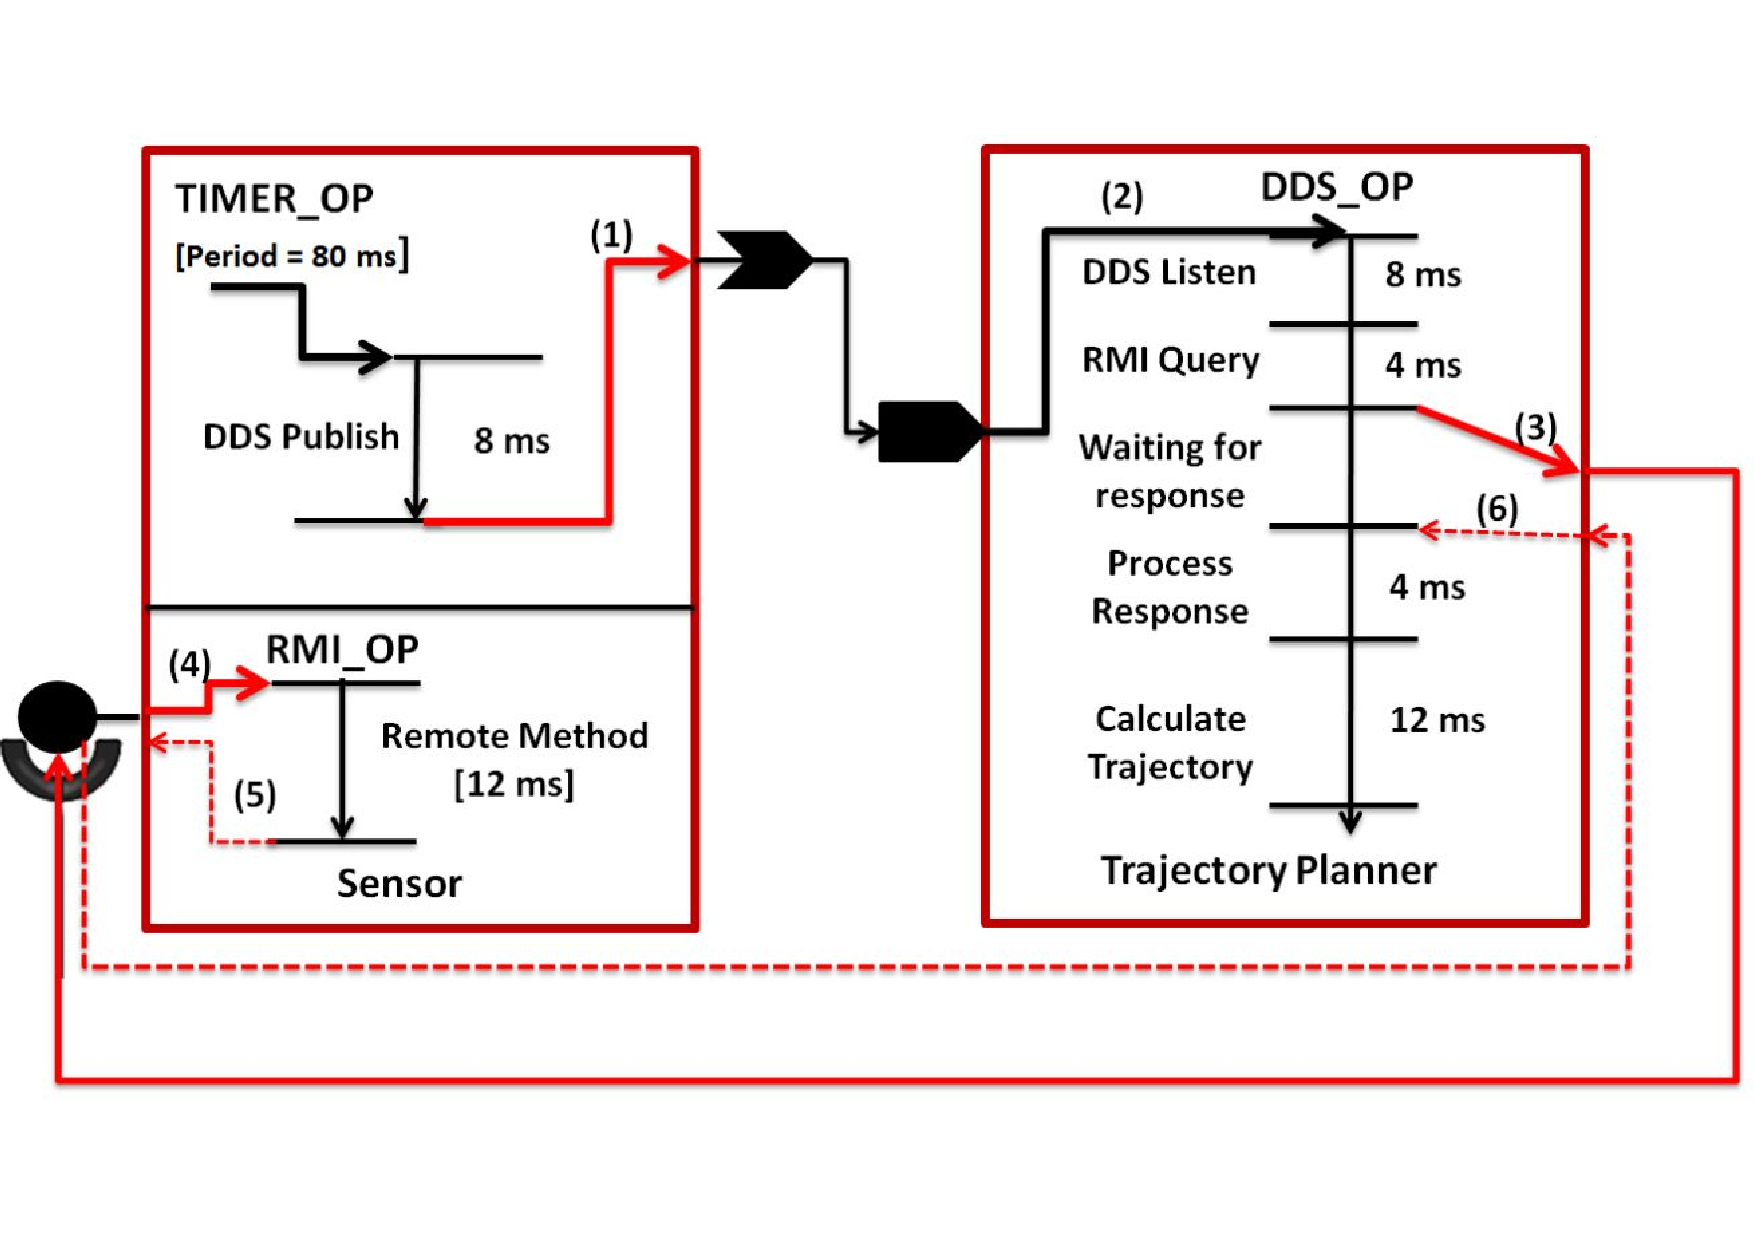
\includegraphics[width=0.88\textwidth]{./figs/CPN_TPA}
\caption{Trajectory Planning Application}
\label{fig:tpa}
\vspace{-0.2in}
\end{figure}
%\vspace{0.1in}

\begin{figure}[ht]
\centering
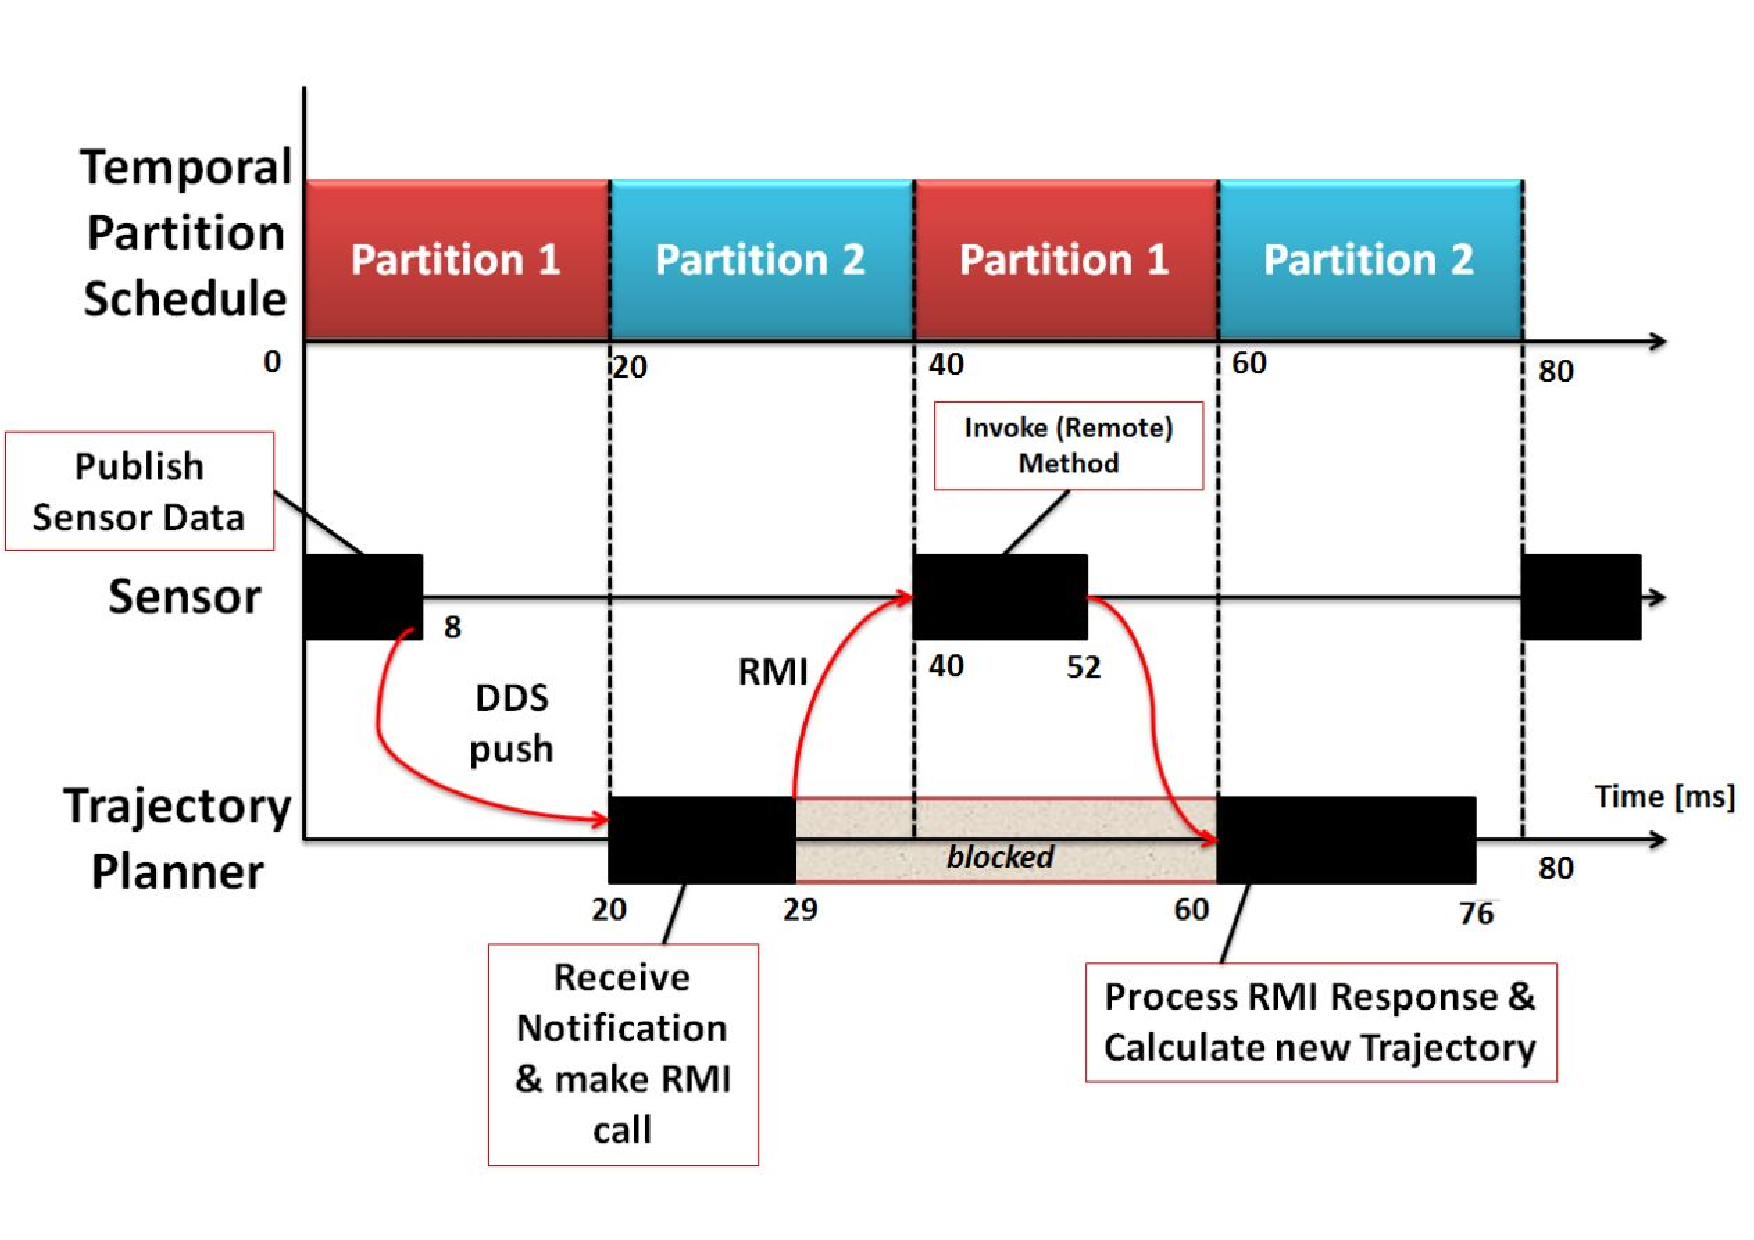
\includegraphics[width=0.8\textwidth]{./figs/CPN_TPA_TD}
\caption{Timing Diagram for Trajectory Planning}
\label{fig:tpa_td}
\vspace{-0.2in}
\end{figure}
\vspace{0.1in}

Figure \ref{fig:tpa_td} shows the partition schedule and temporal behavior considered. The sensor component operates on partition 1, and the trajectory planner operates on partition 2. Both partitions have a duration of 20 ms and a period of 40 ms. The sensor component is associated with a periodic timer that fires every 80 ms. When this timer expires, the sensor component publishes on a notification topic. Accounting for network latencies, the analysis assumes that this task does not take more than 8 ms. Once the notification is sent out, the sensor component becomes passive. With DDS push semantics, this notification manifests itself as a DDS operation on the trajectory planner's message queue. When partition 2 becomes active, the trajectory planner component receives the notification is has subscribed to, after which it makes an RMI call to the sensor component to obtain the updated sensor values. After the RMI call is made, this component blocks for the remainder of the partition. When the sensor component is scheduled again, it services the RMI request and sends out the RMI response, effectively unblocking the trajectory planner. Once the new sensor data is retrieved, the trajectory planner calculates a new trajectory for the satellite node. 

\vspace{0.1in}
\noindent\textbf{Location:}\\
\texttt{\$F6IAP/f6mde/f6ml/IM/samples/CPNAnalysis\_Samples/ \\ Trajectory\_Planning\_Application}
   \texttt{/Scenario\_1\_RMI\_Blocking\_Delay/}
	
\section{Adding BusinessLogic Atoms to Component Ports}

In the F6ML model of the application, \emph{BusinessLogic} atoms can be added to component ports exposed in the Component Implementation. BusinessLogic atoms represent the timing specifications for the operations that are implemented by the component port. For instance - In order to model the timing specification of a timer operation in a component, the first step is to:
\begin{enumerate}
\item Drag a new BusinessLogic atom to the canvas from the Development aspect in the Part Browser inside the Component Implementation.
\item Connect this atom to a \emph{Timer} port exposed on the instance of the Component Definition.
\item The Operations attribute of this BusinessLogic atom represents the timing specification of the timer operation.
\end{enumerate}

Figure \ref{fig:tpa_timerbl} shows a BusinessLogic atom called \emph{Timer\_BL} connected to a timer port \emph{Publish\_Timer} in the Sensor component. Note that the BusinessLogic atom is only visible in the \emph{Development} aspect inside Component Implementation.

\begin{figure}[ht]
\centering
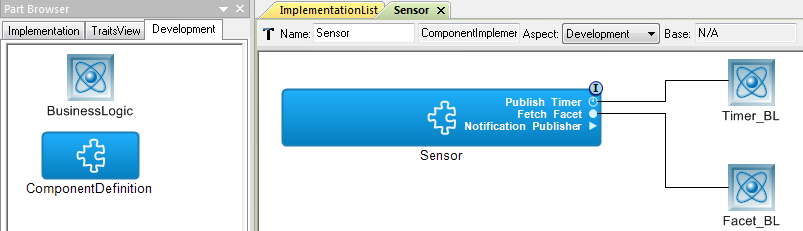
\includegraphics[width=0.99\textwidth]{./figs/TPA_TIMERBL}
\caption{Connecting a BusinessLogic atom to a Component Port}
\label{fig:tpa_timerbl}
\vspace{-0.2in}
\end{figure}
\vspace{0.1in}

\section{ANTLR 4 Grammar for Component Operations}

The timing behavior for business logic of component operations is expressed in the \emph{Operations} attribute of a BusinessLogic atom. This behavior is modeled using a well-defined ANTLR 4 grammar. This section describes the grammar and how it applied is for the trajectory planning application. 

\subsection{Defining the Timing Specification}

The Operations attribute of a BusinessLogic atom consists of one or more \emph{operations}. Each operation: 
\begin{enumerate}
\item Begins with the keyword \emph{'Do'}, followed by
\item The \emph{name} of the component operation, followed by
\item The \emph{priority} of the component operation, followed by
\item The \emph{deadline} of the component operation.
\item One or more operational steps
\end{enumerate}

Note that the priority and deadline of the operation are specified inside square brackets. This is defined in the grammar in Figure \ref{fig:grammar1}.

The name of the component operation is important. For instance - 
\begin{itemize}
\item Every timer operation needs to be called \emph{on\_timer}.
\item Every subscriber operation where the subscriber is configured to be of type \emph{PUSH\_WITHOUT\_INSTANCE\_NOTIFICATIONS} - should be named either \emph{on\_one\_data} or \emph{on\_many\_data}. 
\item Every subscriber operation where the subscriber is configured to be of type \emph{PUSH\_WITH\_INSTANCE\_NOTIFICATIONS} - should be named either \emph{on\_one\_update} or \emph{on\_many\_updates}. 
\item Every facet operation name must match one of the methods defined in the interface that refers the connected facet. 
\end{itemize}

If any of these rules are not followed, the CPNGenerator interpreter will provide a GME Console Error detailing the issue.

\begin{figure}[ht]
\centering
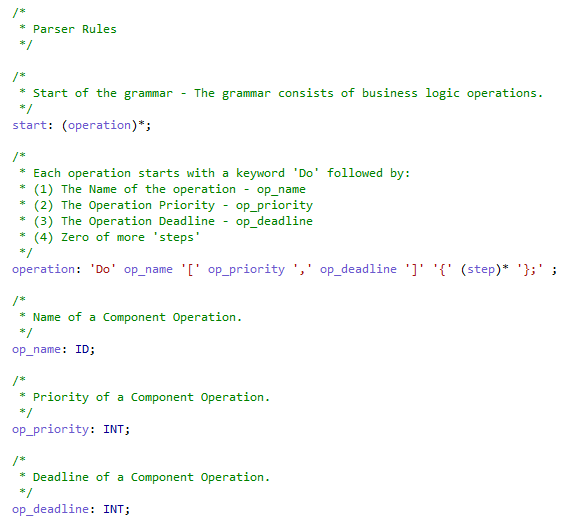
\includegraphics[width=0.99\textwidth]{./figs/Grammar_1}
\caption{Modeling Component Operations}
\label{fig:grammar1}
\vspace{-0.2in}
\end{figure}
\vspace{0.1in}

Note that BusinessLogic atoms can only be connected to the following ports: 
\begin{itemize}
\item Timer ports
\item Push Subscriber ports 
\item Facets
\item AMI Receptacles - describing AMI callback operations
\end{itemize}

As mentioned earlier, every operation is described by the sequence of steps executed in the business logic. As shown in Figure \ref{fig:grammar2}, an operational step can be a (1) Fragment of code, (2) RMI call, (3) AMI call, (4) DDS Publish, (5) DDS Pull Subscribe, (6) DDS Push Subscribe or a (7) Control Loop.

\begin{figure}[ht]
\centering
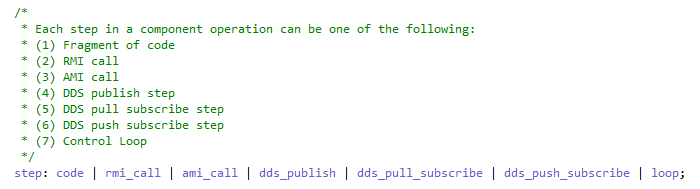
\includegraphics[width=0.99\textwidth]{./figs/Grammar_2}
\caption{Operational steps}
\label{fig:grammar2}
\vspace{-0.2in}
\end{figure}
\vspace{0.1in}

Figures \ref{fig:code_fragment}. \ref{fig:grammar3}, \ref{fig:grammar4}, \ref{fig:grammar5}, \ref{fig:grammar6} and \ref{fig:grammar7} show how the different operational steps are defined in the Business Logic grammar. 

\subsection{Code Fragment}

\begin{figure}[ht]
\centering
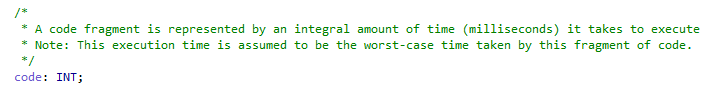
\includegraphics[width=0.99\textwidth]{./figs/Grammar_code}
\caption{Code Fragment}
\label{fig:code_fragment}
\vspace{-0.2in}
\end{figure}
\vspace{0.1in}



\subsection{RMI call}

\begin{figure}[ht]
\centering
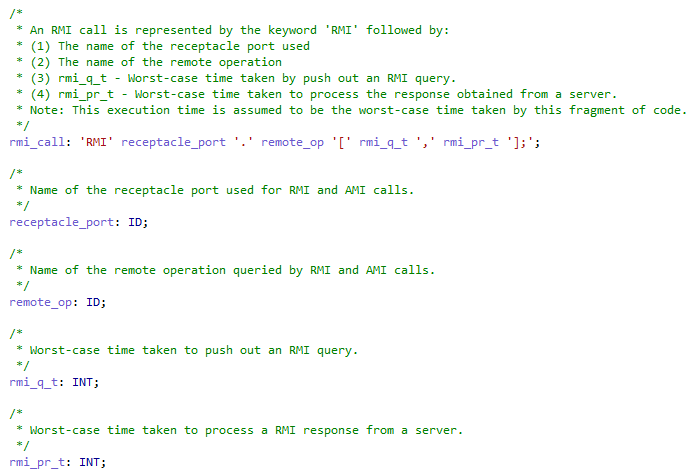
\includegraphics[width=0.99\textwidth]{./figs/Grammar_3}
\caption{RMI call}
\label{fig:grammar3}
\vspace{-0.2in}
\end{figure}
\vspace{0.1in}

\subsection{AMI call}

\begin{figure}[ht]
\centering
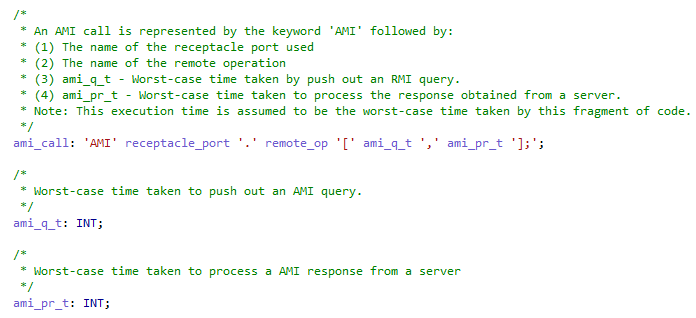
\includegraphics[width=0.99\textwidth]{./figs/Grammar_4}
\caption{AMI call}
\label{fig:grammar4}
\vspace{-0.2in}
\end{figure}
\vspace{0.1in}

\subsection{DDS Publish}

\begin{figure}[ht]
\centering
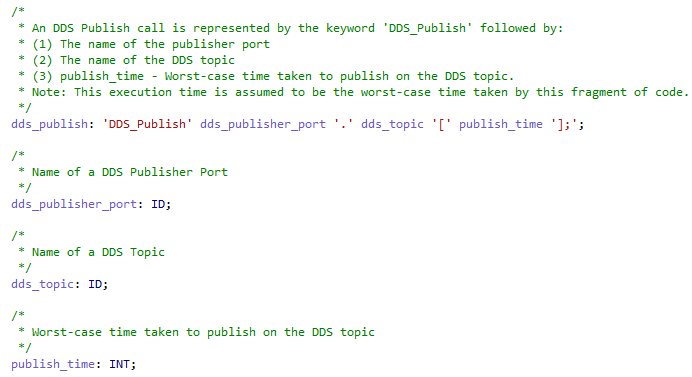
\includegraphics[width=0.99\textwidth]{./figs/Grammar_5}
\caption{DDS Publish call}
\label{fig:grammar5}
\vspace{-0.2in}
\end{figure}
\vspace{0.1in}

\newpage

\subsection{DDS Subscribe}

\begin{figure}[ht]
\centering
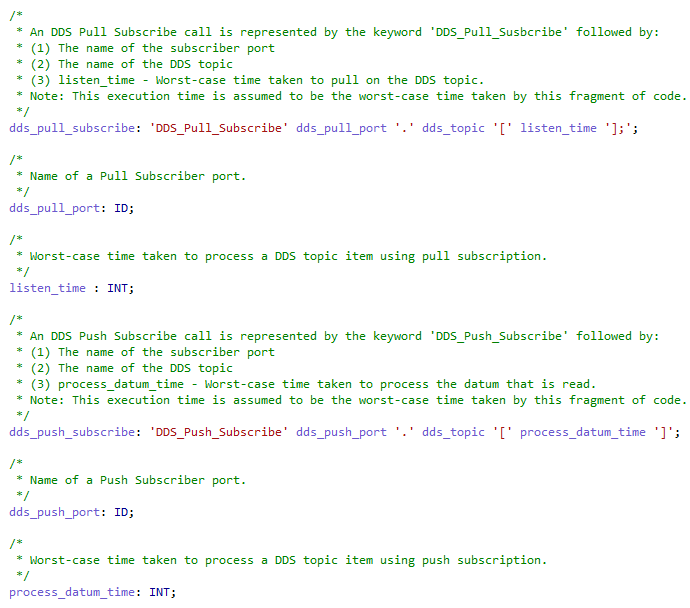
\includegraphics[width=0.99\textwidth]{./figs/Grammar_6}
\caption{DDS Subscribe calls}
\label{fig:grammar6}
\vspace{-0.2in}
\end{figure}
\vspace{0.1in}

\subsection{Control Loops}

\begin{figure}[ht]
\centering
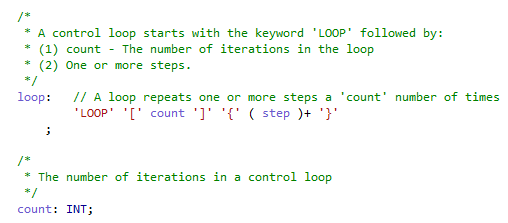
\includegraphics[width=0.70\textwidth]{./figs/Grammar_7}
\caption{Control Loops in the Business Logic}
\label{fig:grammar7}
\vspace{-0.2in}
\end{figure}
\vspace{0.1in}


\section{Modeling the Sensor and Trajectory Planner Operations}

As shown in Figure \ref{fig:tpa}, the user needs to model three component operations - the timer operation on the Sensor, the facet operation on the Sensor and the DDS Push Subscribe operation on the Trajectory Planner. 

\subsection{Sensor Timer Operation}

\begin{figure}[ht]
\centering
\includegraphics[width=0.75\textwidth]{./figs/tpa_timerop}
\caption{Sensor Timer Operation}
\label{fig:tpa_timer}
\vspace{-0.2in}
\end{figure}
\vspace{0.1in}

\subsection{Sensor Facet Operation}

\begin{figure}[ht]
\centering
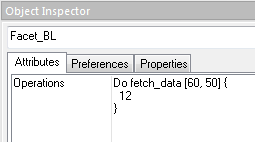
\includegraphics[width=0.60\textwidth]{./figs/TPA_FACETOP}
\caption{Sensor Facet Operation}
\label{fig:tpa_facet}
\vspace{-0.2in}
\end{figure}
\vspace{0.1in}

\subsection{Trajectory Planner DDS Push Subscribe Operation}

\begin{figure}[ht]
\centering
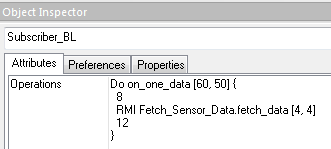
\includegraphics[width=0.70\textwidth]{./figs/TPA_PSH}
\caption{Trajectory Planner DDS Push Subscribe Operation}
\label{fig:tpa_psh}
\vspace{-0.2in}
\end{figure}
\vspace{0.1in}




\chapter{Using the CPNGenerator Interpreter}

Once the component business logic operations are modeled, it is time to generate an analysis model for the application. 

\emph{Reminder:} In order for this section to be useful, a clean installation of the CPN Tools 4 Tool Suite is required. 

From the Software Deployment aspect in the F6ML model, click on the CPNGenerator interpreter (Figure \ref{fig:interpreter}).

\begin{figure}[ht]
\centering
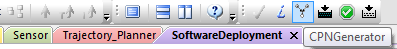
\includegraphics[width=0.80\textwidth]{./figs/interpreter}
\caption{CPNGenerator Interpreter}
\label{fig:interpreter}
\vspace{-0.2in}
\end{figure}
\vspace{0.1in} 

Once the interpreter starts, it prints a sequence of debug messages. These messages are organized as follows: 

\subsection{Application Summary}

For every application, the first set of debug messages shows the following messages for each component: 
\begin{itemize}
\item Component Name, Actor Name, Actor ID, Actor Priority, Node Name
\item Receptacle (if any) Name, Interface Name, Type of Receptacle
\item Facet (if any) Name, Interface Name
\item DDS Publisher Name, Topic Name
\item DDS Subscriber Name, Topic Name, Subscription Type
\end{itemize}

Figure \ref{fig:app_summary_1} shows the application summary for the Trajectory Planning Application: 

\begin{figure}[ht]
\centering
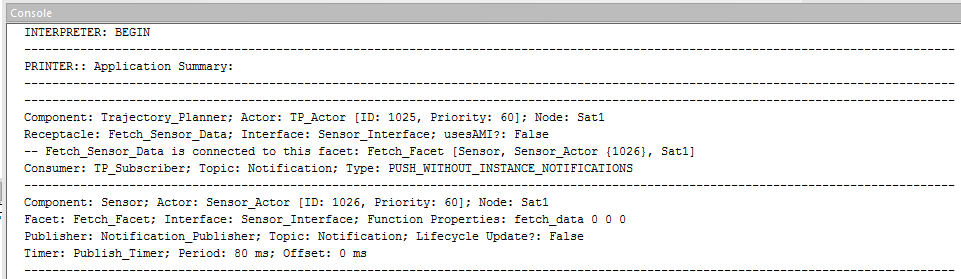
\includegraphics[width=0.99\textwidth]{./figs/app_summary_1}
\caption{Application Summary}
\label{fig:app_summary_1}
\vspace{-0.2in}
\end{figure}
\vspace{0.1in} 

\begin{figure}[ht]
\centering
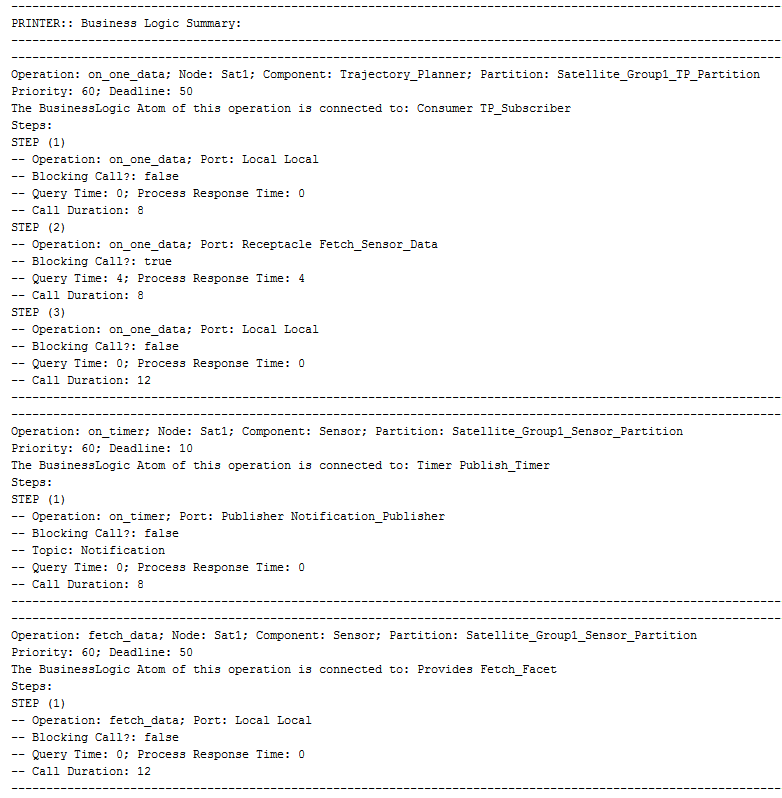
\includegraphics[width=0.8\textwidth]{./figs/app_summary_2}
\caption{Business Logic Summary}
\label{fig:app_summary_2}
\vspace{-0.2in}
\end{figure}
\vspace{0.1in} 

\subsection{Business Logic Summary}
The second set of debug messages shows the summary of every component operation BusinessLogic in the application. This includes: 
\begin{itemize}
\item Operation Name, Node Name, Component Name, Partition Name.
\item Operation Priority, Operation Deadline.
\item Set of Steps in the Component Operation.
\end{itemize}

\newpage

\subsection{Generated CPN files}

The CPNGenerator generates two files for the timing analysis. 
\begin{itemize}
\item CPN\_Analysis\_Model.cpn
\item functions.sml
\end{itemize}

The CPN\_Analysis\_Model.cpn is the main colored petri net file. This is the primary analysis model. The extension .cpn refers to a CPN Tools-based colored petri net. This model is therefore opened by CPN Tools. 

\begin{figure}[ht]
\centering
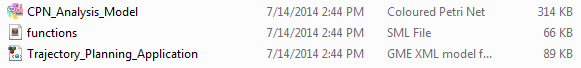
\includegraphics[width=0.9\textwidth]{./figs/generated}
\label{fig:generated}
\vspace{-0.2in}
\end{figure}
\vspace{0.1in} 

In addition, the functions.sml file is standard ML file that contains all of the functions used by transition guards and arc inscriptions in the CPN model.

\begin{figure}[ht]
\centering
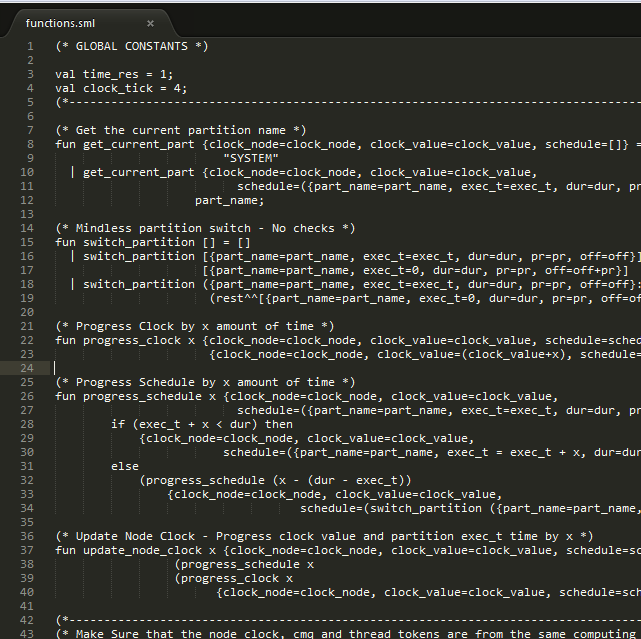
\includegraphics[width=0.9\textwidth]{./figs/functions}
\label{fig:functions}
\vspace{-0.2in}
\end{figure}
\vspace{0.1in} 




\chapter{State Space Analysis}

In order to use the generated .cpn file for state space analysis, preliminary knowledge on (1) the concept of colored petri nets, and (2) the concepts of the CPN Tools 4 Tool Suite. 

Open CPN\_Analysis\_Model.cpn using CPN Tools 4. The Analysis\_Model canvas in the model should look like this:

\begin{figure}[ht]
\centering
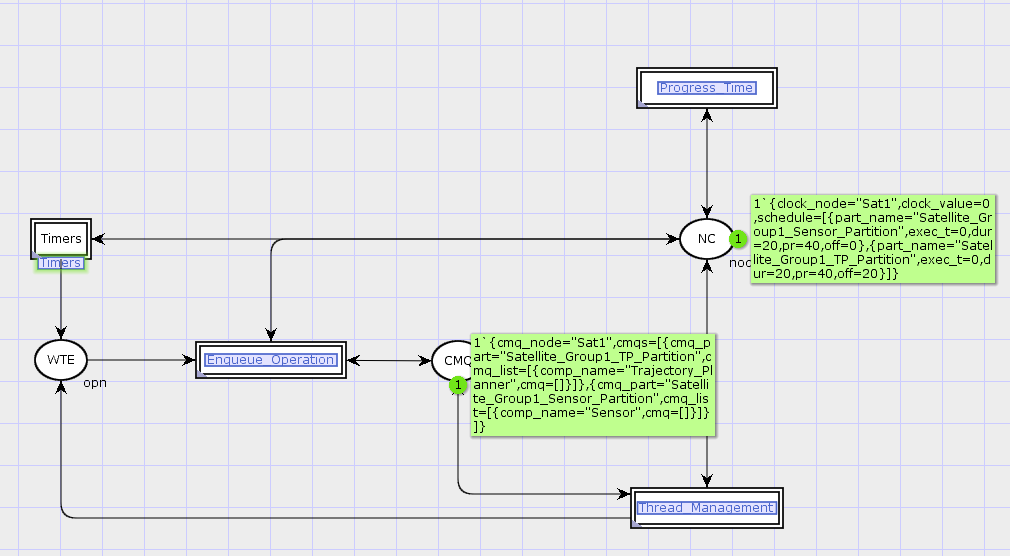
\includegraphics[width=0.9\textwidth]{./figs/Analysis}
\caption{CPN Analysis Model}
\label{fig:analysis}
\vspace{-0.2in}
\end{figure}
\vspace{0.1in} 

The colored petri net tokens in this model are application-specific and created by CPNGenerator when it parses the application. Now drag the State Space Tool onto the canvas. The settings on the state space tool can be set by right clicking on \emph{SS} tool and clicking on \emph{Set Options}. For the trajectory planner application, set the settings as shown in Figure \ref{fig:sss}.

Use the state space tool to generate a bounded state space for the analysis model using the applied settings. A successful bounded state space generation leads to a prompt as shown in Figure \ref{fig:sss}.

Once a bounded state space is generated, it is time to search this state space and obtain useful analysis results. The page Analysis\_Model consists of a set of state space queries generated by CPNGenerator. Use the \emph{ML!} tool (ML evaluate) to evaluate standard ML code (the state space queries).

\begin{figure}[ht]
\centering
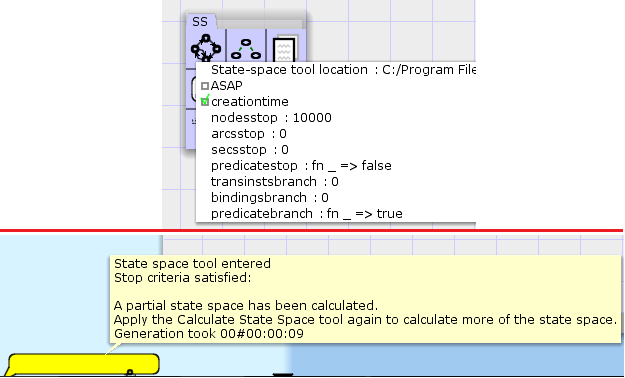
\includegraphics[width=0.9\textwidth]{./figs/SSS}
\caption{State Space Tool}
\label{fig:sss}
\vspace{-0.2in}
\end{figure}
\vspace{0.1in} 

\subsection{Deadline Violation Detection}
Using the \emph{op\_st} and \emph{op\_et} fields of every component operation, the model is capable of identifying deadline violations in component operations that are either currently in progress or waiting in the component message queue. The model essentially takes a snapshot of such cases and records the time stamps. For instance: In Figure \ref{fig:tpa_td}, the \emph{on\_one\_data} on the Trajectory Planner Component starts at time = 20 and completes at time = 76, taking 56 ms accounting for temporal partitioning and the block time due to the remote call. If the deadline for this operation were to be set at 50 ms, the model would take notice of the violation at time = 51. This can also be observed by relying on the simulation tool as there is only one thread execution order for this scenario. Figures \ref{fig:cpn_tpa_dv_marking} and \ref{fig:cpn_tpa_dv_ss} show the observed deadline violation and the state space queries that reinforce the observation. The \emph{SearchNodes} function enables searching parts of the state space and identifying nodes that support a predicate function. In this case, the predicate function obtains state space nodes where a deadline violation is recorded in the \emph{Late\_Op} place. From this subset of nodes, unique deadline violations are identified. A backtrace for the observed violation can be easily obtained by using the \emph{NodesInPath (InitialNode, DestNode)} function that presents an ordered list of state space nodes from the initial node that represents the path taken to reach the violation node.

\begin{figure}[ht]
\centering
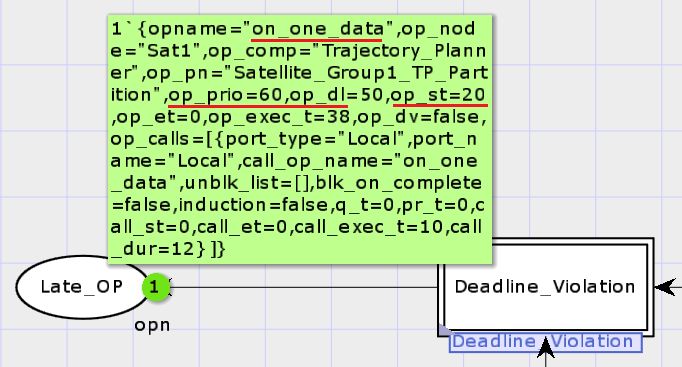
\includegraphics[width=0.60\textwidth]{./figs/cpn_tpa_dv_marking}
\caption{Observed Deadline Violation}
\label{fig:cpn_tpa_dv_marking}
\vspace{-0.2in}
\end{figure}
\vspace{0.1in}

\begin{figure}[ht]
\centering
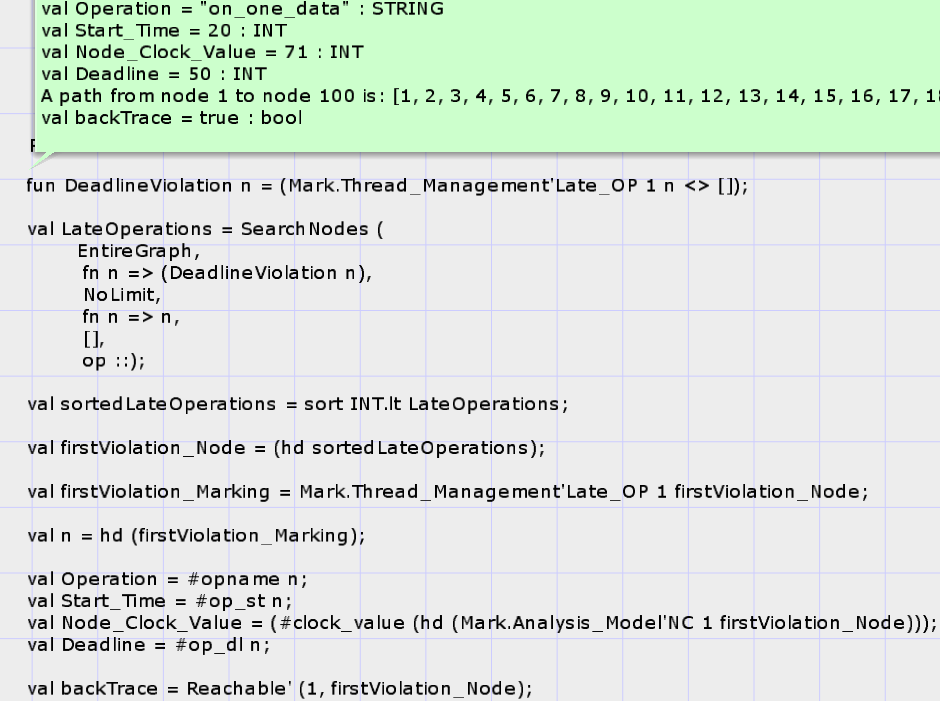
\includegraphics[width=0.99\textwidth]{./figs/cpn_tpa_dv_ss}
\caption{State Space Query for Deadline Violation Detection}
\label{fig:cpn_tpa_dv_ss}
\vspace{-0.2in}
\end{figure}

\subsection{Worst-case Trigger-to-Response Time Calculation}

As component operations run to completion, the analysis model keeps track of operation completion using a \emph{COP} place as shown in Figure \ref{fig:cpn_completed_operations}. 

\begin{figure}[ht]
\centering
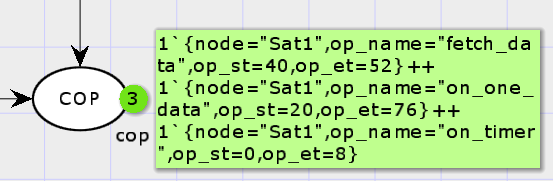
\includegraphics[width=0.60\textwidth]{./figs/cpn_completed_operations}
\caption{Completed Operations}
\label{fig:cpn_completed_operations}
\vspace{-0.2in}
\end{figure}
\vspace{0.1in}

For a known trigger operation and desired response operation, the worst-case trigger-to-response time can also be calculated from the generated state space. This is especially useful when multiple threads of same priority share a partition leading to a tree of possible thread execution orders. Once the necessary partial state space is generated, by using the operation IDs of the trigger and response, the earliest completion of the trigger operation and the latest completion of the response operation within the set period are identified. In the Trajectory Planning application, considering the \emph{on\_timer} to be the trigger and the trajectory planning \emph{on\_one\_data} to be the response, the worst-case response time is found to be 65 ms as shown in Figure \ref{fig:cpn_tpa_trigger_response_time}. Since all of the necessary information is already packed in the state space, variants of such queries can be easily constructed without changing the model.

\begin{figure}[ht]
\centering
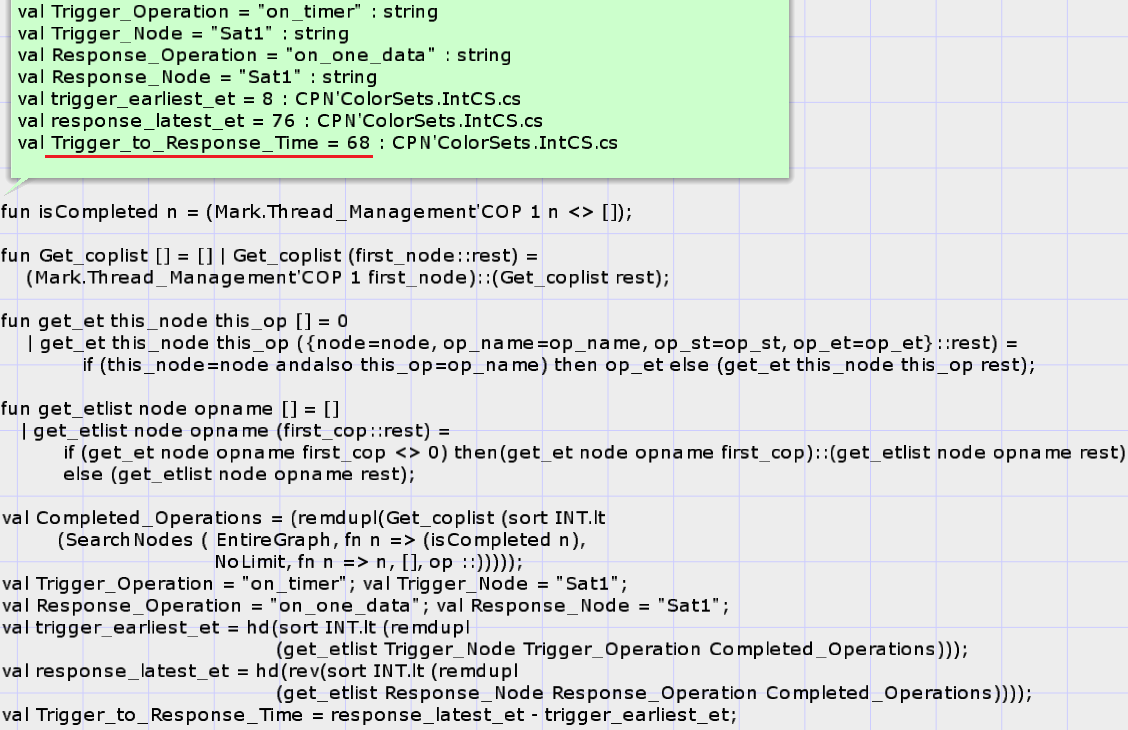
\includegraphics[width=0.99\textwidth]{./figs/cpn_tpa_trigger_response_time}
\caption{Worst-Case Trigger-to-Response Time Calculation}
\label{fig:cpn_tpa_trigger_response_time}
\vspace{-0.2in}
\end{figure}
\vspace{0.1in}

It must be noted here that understanding the state space queries requires knowledge on standard ML code. Using standard ML, similar queries can be written as auxillary text in the CPN page. 

\chapter{Samples}

\subsection{Periodic AMI operations - Deadline Violation}

\label{sec:AMI}
\noindent\textbf{Description:}\\
The goal of this scenario is to test the utility of the analysis tool in handling AMI calls inside the business logic of component operations. The test consists of two components - a Client and a Server component. The client component is associated with a timer that fires once at every hyperperiod. In the business logic of this timer operation, the Client component makes an AMI call to a provided operation on a remote Server. The client and server are separated by temporal partitions each 50 ms long. Once the client makes an AMI call, the client thread does not block but instead continues with the rest of the timer operation. Meanwhile, the completion of an AMI query of the client side induces a AMI operation on the server side. This operation is run to completion in Partition 2. On completion of the remote method on the server, a callback operation is induced on the client's message queue. When the client is scheduled again, the callback operation is dequeued and completed. The aim of this test is to verify the correctness of the generated CPN and also the correctness of the observed behavior. 

\noindent\textbf{Location:}\\
\texttt{\$F6IAP/f6mde/f6ml/IM/samples/CPNAnalysis\_Samples/ \\ Periodic\_AMI/Deadline\_Violation/}


\noindent\textbf{Expected Results:}\\
The expected results include the following: 
\begin{enumerate}
\item Successfully generate a CPN\_Analysis\_Model and a functions.sml file by using the CPNGenerator interpreter in the modeling tools.
\item The .cpn file is a valid file, i.e., CPN Tools 4 is able to open the colored petri net without any errors.
\item Using the state space tool in CPN Tools, successfully generate a bounded state space - say 10,000 nodes to observe close to 10 hyperperiods of thread activity.
\item Evaluate the deadline monitoring state space query to realize the presence of a deadline violation.
\end{enumerate}

The AMI callback operation on the client side is set with a deadline of 30 ms but the duration of the operation is set to 45 ms to simulate an unexpected delay in completion. On evaluating the deadline monitor in the analysis tool, a violation is observed as soon as the clock of the component node reaches the deadline of the operation. This observation is shown in Figure \ref{fig:Periodic_AMI_DV}.

\begin{figure}[htb]
\centering
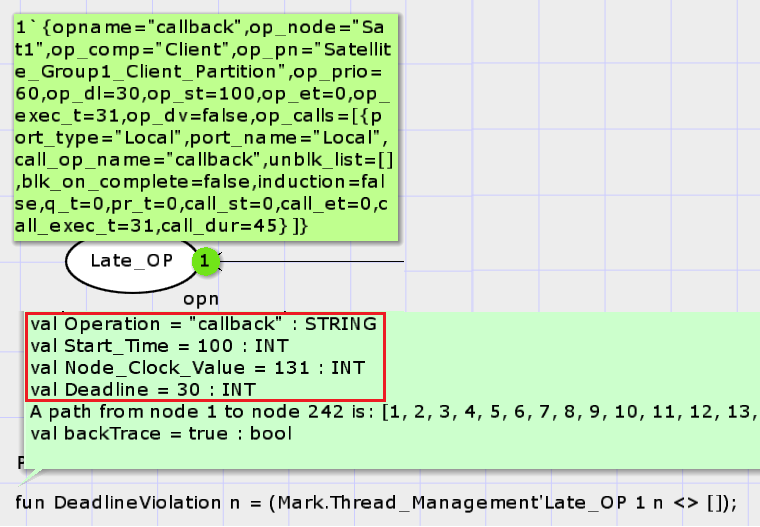
\includegraphics[scale=0.45]{./figs/CPN_Periodic_AMI_DV.png}
\caption{Periodic AMI operations - Deadline Violation}
\label{fig:Periodic_AMI_DV}
\end{figure}

\noindent\textbf{Test Mode:}\\
The mode of testing is manual. Once the colored petri net is generated, the CPN Tools software is used to open the .cpn file, generate a bounded state space and evaluate the generated state space queries to analyze the system.

\noindent\textbf{Prerequisites:}\\
A clean installation of the CPN Tools 4 tool (http://cpntools.org/). This software is required to open, edit, simulate and analyze the generated colored petri nets. 

\subsection{Periodic AMI operations - No Deadline Violation}
\noindent\textbf{Description:}\\
The component assembly of this scenario is identical to \ref{sec:AMI}. However, the duration of the callback operation is reduced to 10 ms and its deadline increased to 60 ms. This motivation for this change is to relax the strictness of the timing specification to allow for timely completion of the scheduled operations. 

\noindent\textbf{Location:}\\
\texttt{\$F6IAP/f6mde/f6ml/IM/samples/CPNAnalysis\_Samples/ \\ Periodic\_AMI/No\_Deadline\_Violation/}


\noindent\textbf{Expected Results:}\\

The expected results include the following: 
\begin{enumerate}
\item Successfully generate a CPN\_Analysis\_Model and a functions.sml file by using the CPNGenerator interpreter in the modeling tools.
\item The .cpn file is a valid file, i.e., CPN Tools 4 is able to open the colored petri net without any errors.
\item Using the state space tool in CPN Tools, successfully generate a bounded state space - say 10,000 nodes to observe close to 10 hyperperiods of thread activity.
\item Evaluate the deadline monitoring state space query to realize the absence of any deadline violations.
\end{enumerate}

The callback operation is enqueued at the same time as in the previous case but only takes 10 ms to complete. Even with the periodicity of the timer triggering new AMI operations, the system remains stable without any deadline violations for the observed duration of time. The state space query produces a negative result in identifying a deadline violation within the observed state space. 

\noindent\textbf{Test Mode:}\\
The mode of testing is manual. Once the colored petri net is generated, the CPN Tools software is used to open the .cpn file, generate a bounded state space and evaluate the generated state space queries to analyze the system.

\noindent\textbf{Prerequisites:}\\
A clean installation of the CPN Tools 4 tool (http://cpntools.org/). This software is required to open, edit, simulate and analyze the generated colored petri nets. 

\subsection{Periodic RMI operations - Deadline Violation}
\label{sec:RMI}

\noindent\textbf{Description:}\\
The goal of this scenario is to test the utility of the analysis tool in handling RMI calls inside the business logic of component operations. The test consists of two components - a Client and a Server component. The client component is associated with a timer that fires once at every hyperperiod. In the business logic of this timer operation, the Client component makes an RMI call to a provided operation on a remote Server. The client and server are separated by temporal partitions each 50 ms long. Once the client makes an RMI call, the client thread starts blocking till the server thread on completes executing the remote method and unblocks the client thread. The deadline of the timer operation is set to 120 ms. The timer fires at time 0 and starts blocking after the RMI call is made. There is no further activity in this partition. At time 50, the server thread is scheduled to execute the RMI operation induced on the server message queue. The server thread executes this operation to completion taking 30 ms, unblocking the client. The client thread however does not get scheduled again till time 100. If the post-processing time for the RMI query and further calculations made on the client exceed the deadline of the timer operation, then a client-side deadline violation is observed.

\noindent\textbf{Location:}\\
\texttt{\$F6IAP/f6mde/f6ml/IM/samples/CPNAnalysis\_Samples/ \\ Periodic\_RMI/Deadline\_Violation/}

\noindent\textbf{Expected Results:}\\

The expected results include the following: 

\begin{enumerate}
\item Successfully generate a CPN\_Analysis\_Model and a functions.sml file by using the CPNGenerator interpreter in the modeling tools.
\item The .cpn file is a valid file, i.e., CPN Tools 4 is able to open the colored petri net without any errors.
\item Using the state space tool in CPN Tools, successfully generate a bounded state space - say 10,000 nodes to observe close to 10 hyperperiods of thread activity.
\item Evaluate the deadline monitoring state space query to realize the presence of a deadline violation.
\end{enumerate}

The RMI call blocks the client thread till time 100 ms. When the client is scheduled again, the amount of work required to complete the client timer operation (26 ms) exceeds the deadline of this operation (120 ms) and so a deadline violation is observed at time 121 ms. This observation can be seen in Figure \ref{fig:Periodic_RMI_DV}

\begin{figure}[htb]
\centering
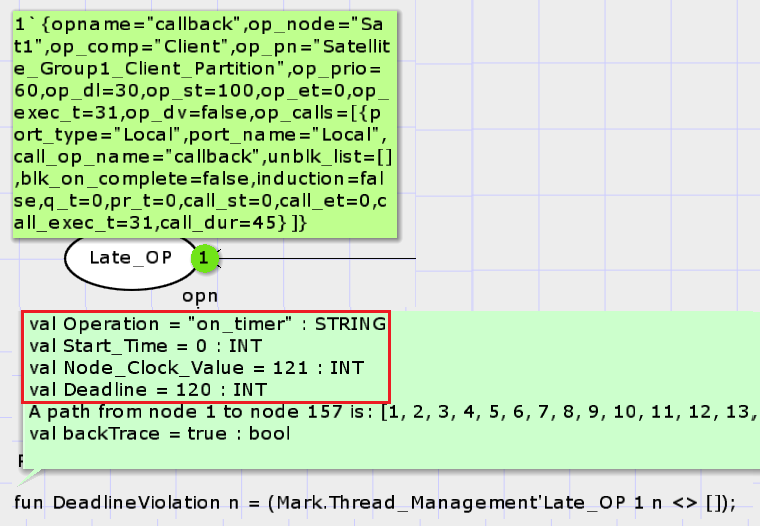
\includegraphics[scale=0.45]{./figs/CPN_Periodic_RMI_DV.png}
\caption{Periodic RMI operations - Deadline Violation}
\label{fig:Periodic_RMI_DV}
\end{figure}

\noindent\textbf{Test Mode:}\\
The mode of testing is manual. Once the colored petri net is generated, the CPN Tools software is used to open the .cpn file, generate a bounded state space and evaluate the generated state space queries to analyze the system.

\noindent\textbf{Prerequisites:}\\
A clean installation of the CPN Tools 4 tool (http://cpntools.org/). This software is required to open, edit, simulate and analyze the generated colored petri nets. 

\subsection{Periodic RMI operations - No Deadline Violation}

\noindent\textbf{Description:}\\
The component assembly of this scenario is identical to \ref{sec:RMI}. However, the deadline of the client timer operation is relaxed by 10 ms to provide for a timely completion. 

\noindent\textbf{Location:}\\
\texttt{\$F6IAP/f6mde/f6ml/IM/samples/CPNAnalysis\_Samples/ \\ Periodic\_RMI/No\_Deadline\_Violation/}

\noindent\textbf{Expected Results:}\\
The expected results include the following: 
\begin{enumerate}
\item Successfully generate a CPN\_Analysis\_Model and a functions.sml file by using the CPNGenerator interpreter in the modeling tools.
\item The .cpn file is a valid file, i.e., CPN Tools 4 is able to open the colored petri net without any errors.
\item Using the state space tool in CPN Tools, successfully generate a bounded state space - say 10,000 nodes to observe close to 10 hyperperiods of thread activity.
\item Evaluate the deadline monitoring state space query to realize the absence of any deadline violations.
\end{enumerate}
The client timer operation completes at time 126 ms which is 4 ms short of its deadline and so no deadline violations are observed and the system is stable. 

\noindent\textbf{Test Mode:}\\
The mode of testing is manual. Once the colored petri net is generated, the CPN Tools software is used to open the .cpn file, generate a bounded state space and evaluate the generated state space queries to analyze the system.

\noindent\textbf{Prerequisites:}\\
A clean installation of the CPN Tools 4 tool (http://cpntools.org/). This software is required to open, edit, simulate and analyze the generated colored petri nets. 

\subsection{Trajectory Planning Application - Deadline Violation due to RMI blocking delay}
\label{sec:TPA_S1}

\noindent\textbf{Description:}\\
The component assembly for this application consists of two components: A \emph{Sensor} component and a \emph{Trajectory Planner} component. The Sensor component periodically publishes on a trigger topic, notifying the Trajectory Planner of the existence of new sensor data. Once the notification is received, the Trajectory Planner makes an RMI call to retrieve the data structure of sensor values. Using the updated sensor values, the Trajectory Planner calculates a new trajectory for the satellite. 

Figure \ref{fig:TPA_TD} shows the partition schedule and temporal behavior considered. The sensor component operates on partition 1, and the trajectory planner operates on partition 2. Both partitions have a duration of 20 ms and a period of 40 ms. The sensor component is associated with a periodic timer that fires every 80 ms. When this timer expires, the sensor component publishes on a notification topic. Accounting for network latencies, the analysis assumes that this task does not take more than 8 ms. Once the notification is sent out, the sensor component becomes passive. With DDS push semantics, this notification manifests itself as a DDS operation on the trajectory planner's message queue. When partition 2 becomes active, the trajectory planner component receives the notification is has subscribed to, after which it makes an RMI call to the sensor component to obtain the updated sensor values. After the RMI call is made, this component blocks for the remainder of the partition. When the sensor component is scheduled again, it services the RMI request and sends out the RMI response, effectively unblocking the trajectory planner. Once the new sensor data is retrieved, the trajectory planner calculates a new trajectory for the satellite node.

While modeling this application using the modeling tools, BusinessLogic atoms are connected to appropriate ports in each Component's Implementation and the timing specification for the different operations are correctly written. Once the Business Logic of the component operations are correctly configured, the CPNGenerator Interpreter is used to generate a CPN Analysis Model. The interpreter generates two files: a CPN\_Analysis\_Model.cpn and a functions.sml file.  

The .cpn file is an analyzable colored petri net. Using CPN Tools 4, simulation and state space-based analysis are carried out on the generated net. This particular scenario shows the utility of the analysis tool in identifying missed deadlines in component operations. In this case, if the Trajectory Planner component thread blocks on the RMI call for longer than its configured deadline, the analysis tool identifies the missed deadline and provides a backtrace of state space nodes that lead to a deadline violation. 

\begin{figure}
        \centering
        \begin{subfigure}[b]{0.5\textwidth}
                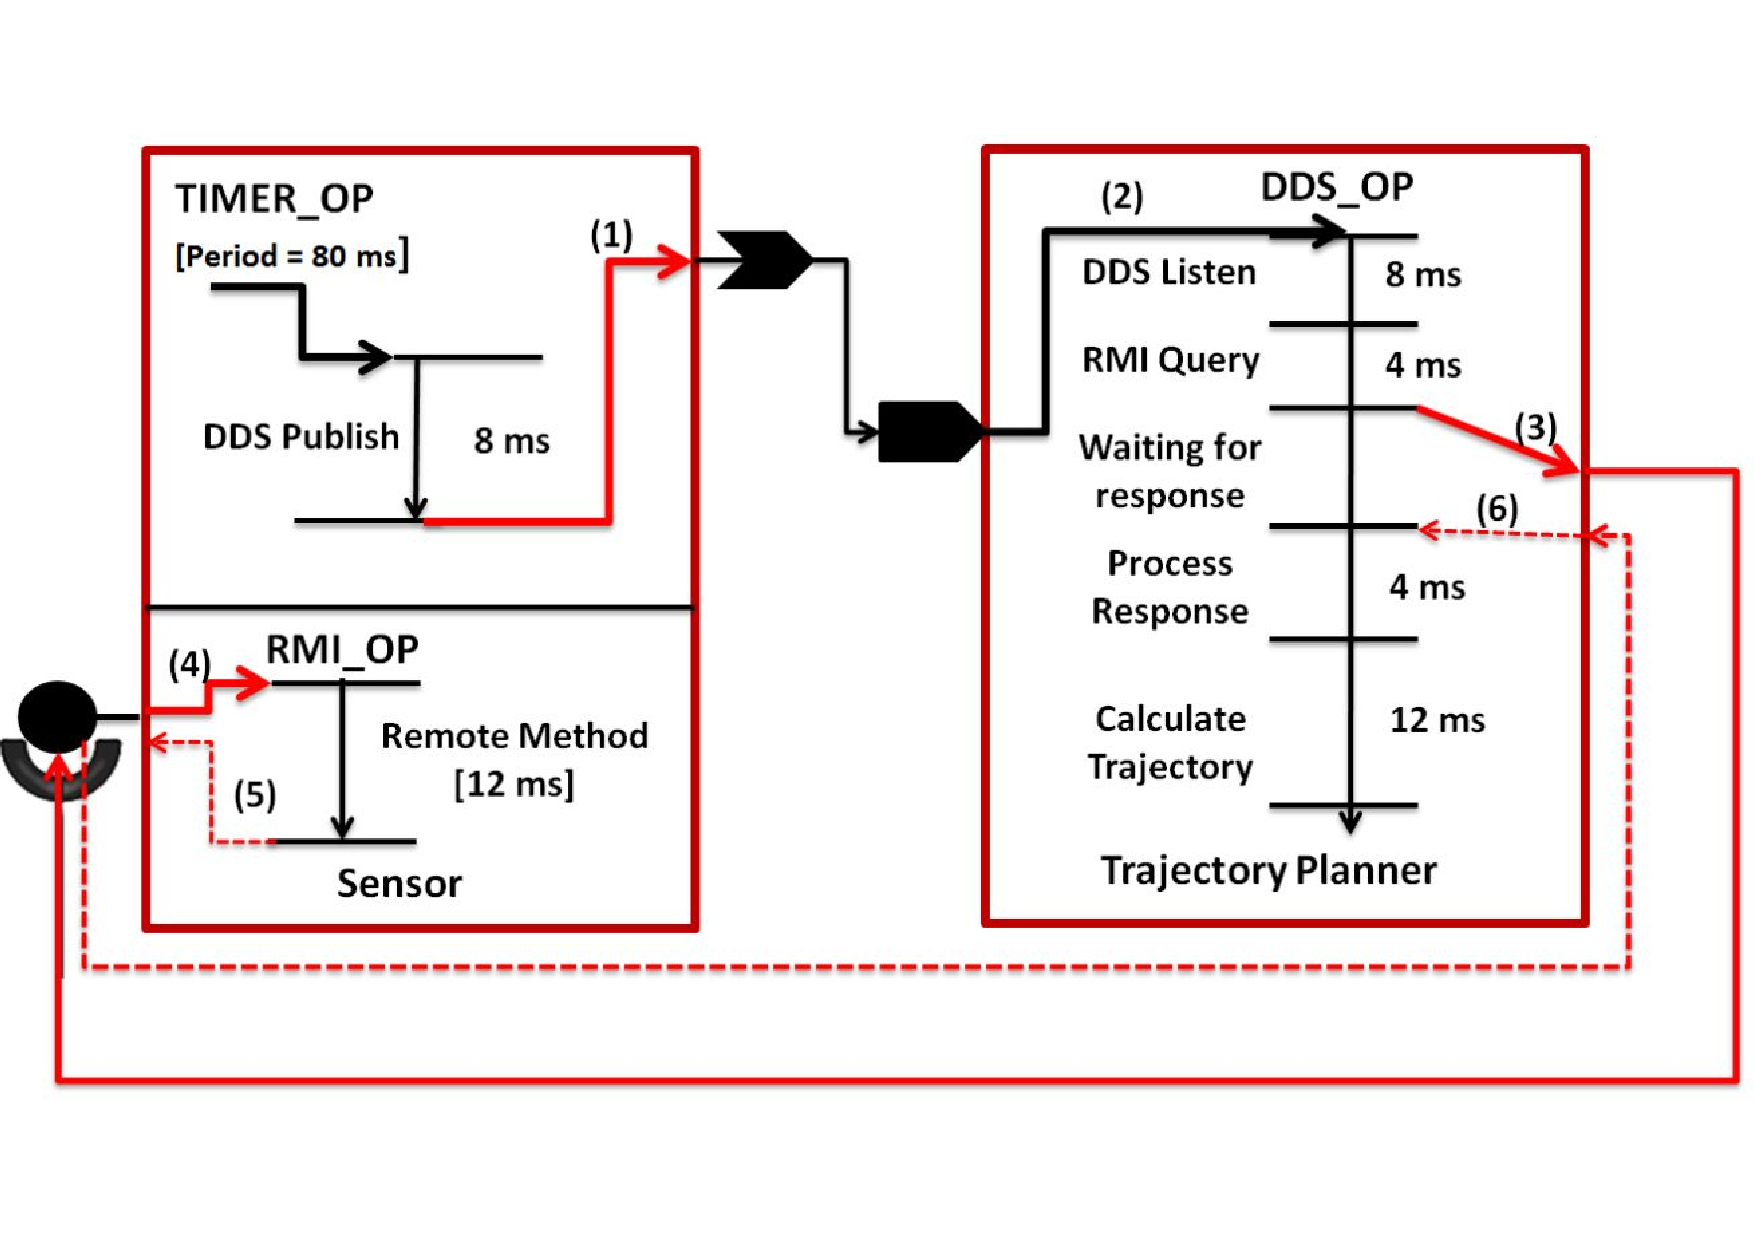
\includegraphics[width=\textwidth]{./figs/CPN_TPA}
                \caption{Component Assembly}
                \label{fig:CA}
        \end{subfigure}%
        \begin{subfigure}[b]{0.5\textwidth}
                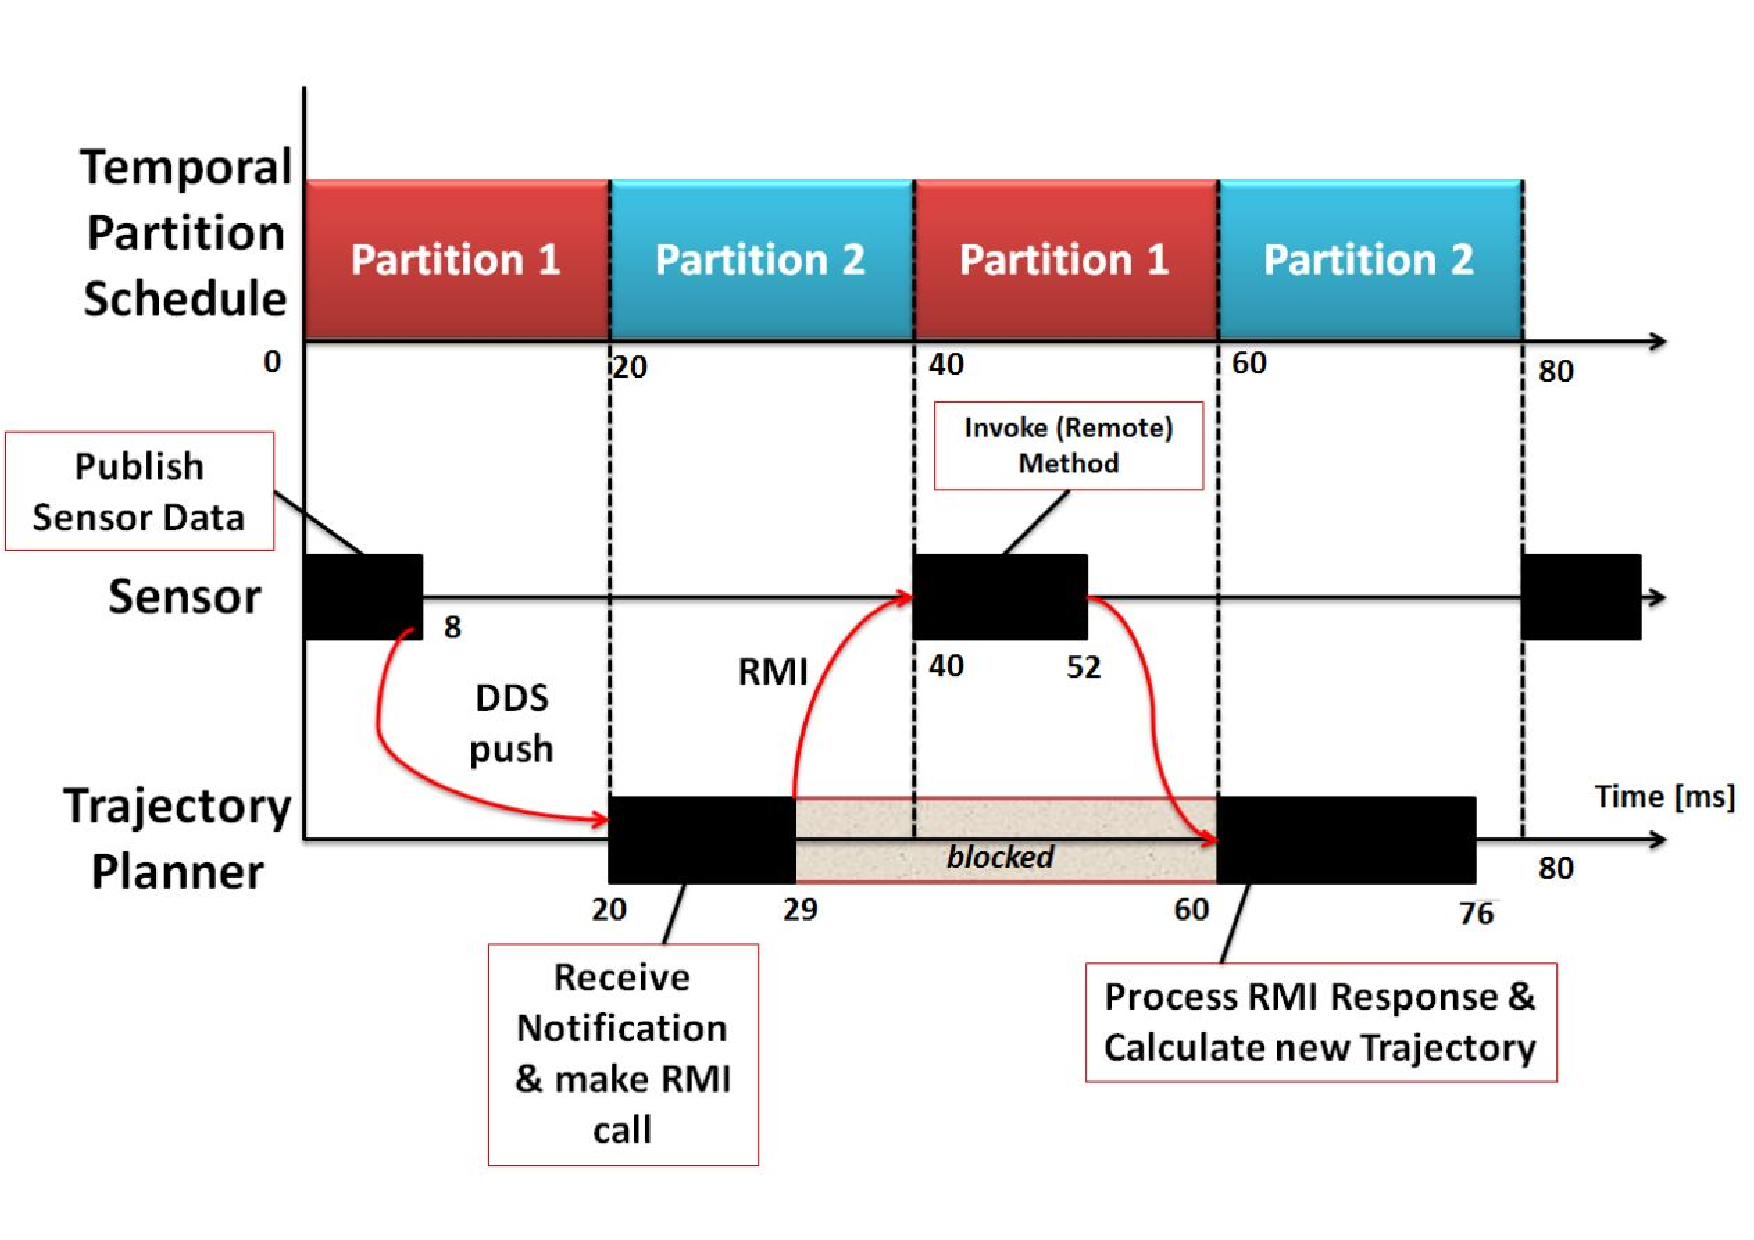
\includegraphics[width=\textwidth]{./figs/CPN_TPA_TD}
                \caption{Timing Diagram}
                \label{fig:TPA_TD}
        \end{subfigure}
        \caption{Trajectory Planning Application}\label{fig:TPA}
\end{figure}

\noindent\textbf{Location:}\\
\texttt{\$F6IAP/f6mde/f6ml/IM/samples/CPNAnalysis\_Samples/ \\ Trajectory\_Planning\_Application}
   \texttt{/Scenario\_1\_RMI\_Blocking\_Delay/}

\noindent\textbf{Expected Results:}\\

The expected results include the following: 
\begin{enumerate}
\item Successfully generate a CPN\_Analysis\_Model and a functions.sml file by using the CPNGenerator interpreter in the modeling tools.
\item The .cpn file is a valid file, i.e., CPN Tools 4 is able to open the colored petri net without any errors.
\item Using the state space tool in CPN Tools, successfully generate a bounded state space - say 10,000 nodes to observe close to 10 hyperperiods of thread activity.
\item Evaluate the deadline monitoring state space query to realize the presence of a deadline violation.
\end{enumerate}
The deadline for the DDS push subscribe operation of the Trajectory Planner is set to 50 ms. This operation starts at a time stamp of 20 ms (at the start of Partition 2). However this operation does not complete till time stamp 76 as shown in \ref{fig:TPA_TD}. This missed deadline is observed as the result of evaluating the state space query.

\noindent\textbf{Test Mode:}\\
The mode of testing is manual. Once the colored petri net is generated, the CPN Tools software is used to open the .cpn file, generate a bounded state space and evaluate the generated state space queries to analyze the system.

\noindent\textbf{Prerequisites:}\\
A clean installation of the CPN Tools 4 tool (http://cpntools.org/). This software is required to open, edit, simulate and analyze the generated colored petri nets. 


\subsection{Trajectory Planning Application - Deadline Violation due to high frequency of timer expiry}

\noindent\textbf{Description:}\\
The component assembly of this scenario is identical to the setup in \ref{sec:TPA_S1}. The frequency of the timer that triggers the Sensor to publish notifications is increased by 8 times. Instead of a period of 80 ms, the timer now has a period of 10 ms. Each timer leads to an infrastructural operation in the Sensor's message queue. Each of these operations has a strict deadline. If the timer expiry is not handled in time, the operations that are enqueued in message queue every 10 ms miss the configured deadline eventually. The analysis aims to identify a deadline violations that are caused by such frequent timer operation requests. 

\noindent\textbf{Location:}\\
\texttt{\$F6IAP/f6mde/f6ml/IM/samples/CPNAnalysis\_Samples/ \\ Trajectory\_Planning\_Application}
\texttt{/Scenario\_2\_Timer\_Expiry\_Frequency/}

\noindent\textbf{Expected Results:}\\

The expected results include the following: 
\begin{enumerate}
\item Successfully generate a CPN\_Analysis\_Model and a functions.sml file by using the CPNGenerator interpreter in the modeling tools.
\item The .cpn file is a valid file, i.e., CPN Tools 4 is able to open the colored petri net without any errors.
\item Using the state space tool in CPN Tools, successfully generate a bounded state space - say 10,000 nodes to observe close to 10 hyperperiods of thread activity.
\item Evaluate the deadline monitoring state space query to realize the presence of a deadline violation.
\end{enumerate}

The deadline of each timer operation is set to 10 ms. However, after each timer operation, the Trajectory Planner receives a notification and makes an RMI call to the Sensor, just as in \ref{sec:TPA_S1}. This RMI call manifests as a facet operation on the Sensor. As shown in \ref{fig:TPA_TD}, the Sensor executes the RMI operation at time 40. Therefore, the Sensor is unable to service the intermediate timer expiry at time 40 ms. The expected result of state space analysis is that the tool identifies a missed deadline at time 51 ms. The timer that expired at 40 ms does not get serviced before its deadline, 10 ms. 

\noindent\textbf{Test Mode:}\\
The mode of testing is manual. Once the colored petri net is generated, the CPN Tools software is used to open the .cpn file, generate a bounded state space and evaluate the generated state space queries to analyze the system.

\noindent\textbf{Prerequisites:}\\
A clean installation of the CPN Tools 4 tool (http://cpntools.org/). This software is required to open, edit, simulate and analyze the generated colored petri nets. 

\subsection{Trajectory Planning Application - Deadline Violation due to publish operations in a loop}

\noindent\textbf{Description:}\\
The goal of this scenario is to test the utility of the analysis tool in handling control loops in the business logic. The CPNGenerator interpreter identifies loops in the business logic of component operations and transforms this nature into appropriate colored petri net tokens that can be used for analysis. The component assembly of this test is similar to \ref{sec:TPA_S1}. The business logic of the timer operation is changed such that the DDS publish step is written inside a control loop. 

\noindent\textbf{Location:}\\
\texttt{\$F6IAP/f6mde/f6ml/IM/samples/CPNAnalysis\_Samples/ \\ Trajectory\_Planning\_Application/}
\texttt{Scenario\_3\_Publishing\_in\_a\_loop/}

\noindent\textbf{Expected Results:}\\

The expected results include the following: 
\begin{enumerate}
\item Successfully generate a CPN\_Analysis\_Model and a functions.sml file by using the CPNGenerator interpreter in the modeling tools.
\item The .cpn file is a valid file, i.e., CPN Tools 4 is able to open the colored petri net without any errors.
\item Using the state space tool in CPN Tools, successfully generate a bounded state space - say 10,000 nodes to observe close to 10 hyperperiods of thread activity.
\item Evaluate the deadline monitoring state space query to realize the presence of a deadline violation.
\end{enumerate}

Each operation publishes on the Notification topic thrice inside a control loop. The deadline is this operation is 30 ms but the operation should only take 24 ms. However, there is an unconditional partition switch at time 20 ms after which the Sensor component is scheduled again only at time 40. Therefore even the first timer operation completes only at time 44 ms, leading to a missed deadline. 

\noindent\textbf{Test Mode:}\\
The mode of testing is manual. Once the colored petri net is generated, the CPN Tools software is used to open the .cpn file, generate a bounded state space and evaluate the generated state space queries to analyze the system.

\noindent\textbf{Prerequisites:}\\
A clean installation of the CPN Tools 4 tool (http://cpntools.org/). This software is required to open, edit, simulate and analyze the generated colored petri nets. 

\subsection{Trajectory Planning Application - Multinode scenario}

\noindent\textbf{Description:}\\
The goal of this scenario is to test the utility of the analysis tool in efficiently handling multi-node deployments. The component assembly is identical to \ref{sec:TPA_S1} but the software bundle consists of copies of this application deployed on multiple nodes. 

\noindent\textbf{Location:}\\
\texttt{\$F6IAP/f6mde/f6ml/IM/samples/CPNAnalysis\_Samples/ \\ Trajectory\_Planning\_Application/}
\texttt{Scenario\_4\_Multinode/}

\noindent\textbf{Expected Results:}\\
The deadlines of all operations are set to large enough values that none of the operations miss deadlines. The CPNGenerator generates a valid CPN model with correct tokens for a multi-node scenario. This includes (1) multiple clock and schedule tokens, one for each node, (2) multiple instances of the Sensor and Trajectory Planner threads, one for each node, (3) multiple instances of component message queues for each thread, one for each node, and (4) a timer token for each Sensor component instance in the bundle. Generating a state space of around 50,000 nodes should be sufficient to observe 10 hyperperiods of thread activity on each node. 

\noindent\textbf{Test Mode:}\\
The mode of testing is manual. Once the colored petri net is generated, the CPN Tools software is used to open the .cpn file, generate a bounded state space and evaluate the generated state space queries to analyze the system.

\noindent\textbf{Prerequisites:}\\
A clean installation of the CPN Tools 4 tool (http://cpntools.org/). This software is required to open, edit, simulate and analyze the generated colored petri nets. 

\subsection{Two-way RMI call - Deadlock}
\label{sec:Two_Way_RMI}

\noindent\textbf{Description:}\\
The goal of this scenario is to test the utility of the analysis tool in identifying system deadlocks. The component assembly (Figure \ref{CPN_RMI_DLK}) consists of two components - a client and a server. When a timer expires on the client component, the client thread makes an RMI call to the server component and starts blocking. When the server component services the requested operation, the server makes an RMI call to an exposed operation on the client. The server starts blocking after dispatching this query. Since both the client and server are blocked on each other, the system reaches a state of deadlock.

\noindent\textbf{Location:}\\
\texttt{\$F6IAP/f6mde/f6ml/IM/samples/CPNAnalysis\_Samples/ \\ TwoWay\_RMI\_Deadlock/}

\begin{figure}[htb]
\centering
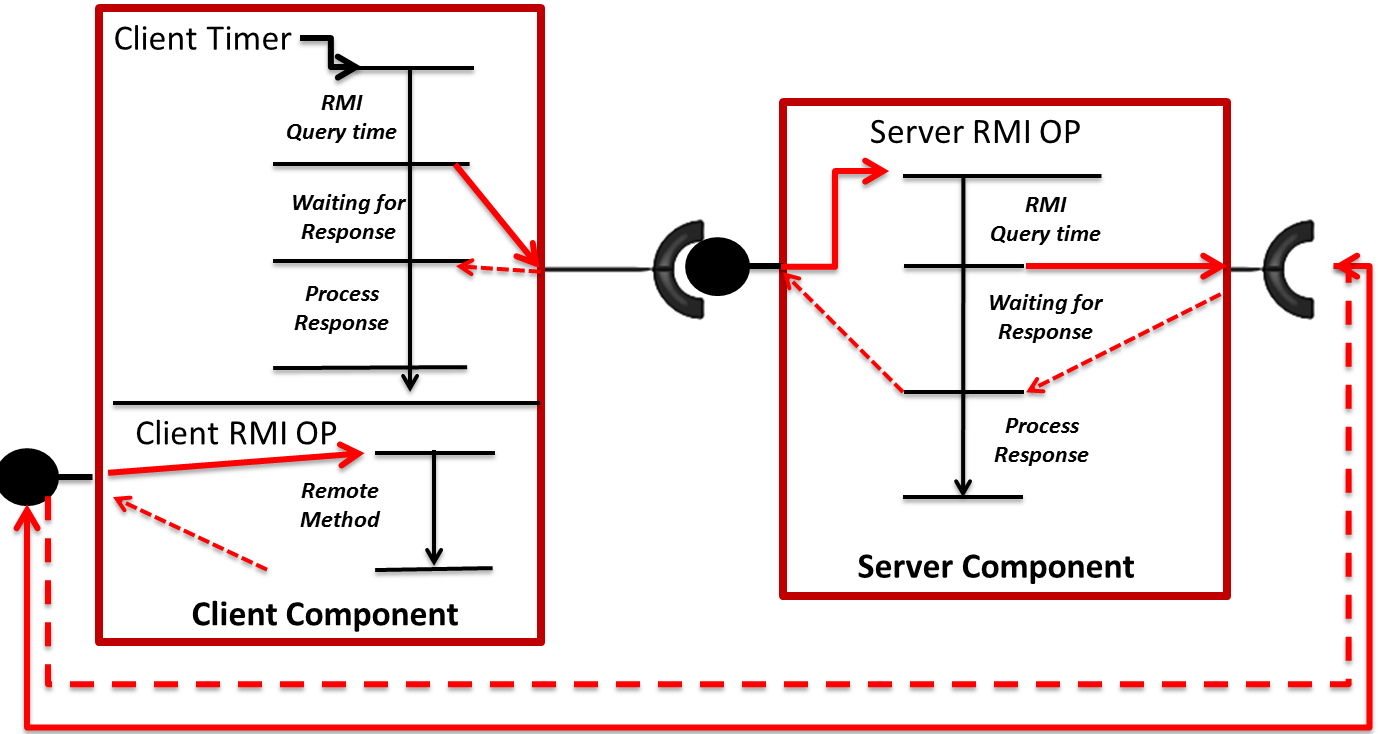
\includegraphics[scale=0.30]{./figs/CPN_RMI_DLK.png}
\caption{Two-Way RMI Deadlock}
\label{fig:CPN_RMI_DLK}
\end{figure}

\noindent\textbf{Expected Results:}\\

The expected results include the following: 
\begin{enumerate}
\item Successfully generate a CPN\_Analysis\_Model and a functions.sml file by using the CPNGenerator interpreter in the modeling tools.
\item The .cpn file is a valid file, i.e., CPN Tools 4 is able to open the colored petri net without any errors.
\item Using the state space tool in CPN Tools, successfully generate a bounded state space - say 10,000 nodes to observe close to 10 hyperperiods of thread activity.
\end{enumerate}

At the end of the first hyperperiod, the client is done dispatching an RMI query to the server and the server is done dispatching an RMI query to the client. Both component threads are blocked on each other and the system reaches a state of deadlock.

\noindent\textbf{Test Mode:}\\
The mode of testing is manual. Once the colored petri net is generated, the CPN Tools software is used to open the .cpn file. Since there is only one possible thread execution order to this scenario, the CPN Tools simulation tool can be used to progress simulation by 100-200 steps. Once the first hyperperiod of activity is complete, the place \emph{BT} indicating the list of blocked thread tokens should hold two tokens - (1) a token representing the client thread blocked on the server and (2) a token representing the server thread blocked on the client. At this point, the system is in the state of deadlock and only the \emph{Progress\_Time} transition should be enabled. 

\noindent\textbf{Prerequisites:}\\
A clean installation of the CPN Tools 4 tool (http://cpntools.org/). This software is required to open, edit, simulate and analyze the generated colored petri nets. 

\end{document}